\section{Direction Fields for First Order Equations}

\noindent
It's impossible to find explicit formulas for solutions of some
differential equations. Even if there are such  formulas, they may be
so complicated that they're useless. In this case we may resort to
graphical or numerical methods to get some idea of how the solutions
of the given equation behave.

 In Section~2.3 we'll take up
the question of existence of solutions of a first order equation
\begin{equation} \label{eq:1.3.1}
y'=f(x,y).
\end{equation}
In this section we'll simply assume that \eqref{eq:1.3.1} has
solutions and discuss a graphical method for approximating them.
In Chapter~3 we discuss numerical methods for obtaining
approximate solutions of \eqref{eq:1.3.1}.

Recall that a solution of \eqref{eq:1.3.1} is a function $y=y(x)$ such
that
$$
y'(x)=f(x,y(x))
$$
for all values of $x$ in some interval, and an integral curve is
either the graph of a solution or is
made up of  segments that are graphs of solutions.
 Therefore, not being able to
solve \eqref{eq:1.3.1} is equivalent to not knowing the equations of
integral curves of \eqref{eq:1.3.1}. However, it's easy to calculate the
slopes of these curves. To be specific, the slope of an integral curve
of \eqref{eq:1.3.1} through a given point $(x_{0},y_{0})$ is given by the
number $f(x_{0},y_{0})$. This is the basis of {\color{blue}\it the method of direction
fields\/}.

If $f$ is defined on a set $R$, we can construct a {\color{blue}\it direction
field \/} for \eqref{eq:1.3.1}  in $R$ by drawing a
short
line segment through each point $(x,y)$ in $R$ with slope $f(x,y)$. Of
course, as a practical matter, we can't actually draw line segments
through {\color{blue}\it every\/} point in $R$;     rather, we must select
a finite
set of points in $R$. For example, suppose   $f$ is defined on the
closed rectangular region
$$
R:\{a\le x\le b,c\le y\le d\}.
$$
Let
$$
a=x_{0}<x_{1}<\cdots<x_{m}=b
$$
be  equally spaced points in $[a,b]$ and
$$
c=y_{0}<y_{1}<\cdots<y_{n}=d
$$
be  equally spaced points in $[c,d]$.
 We say that the points
$$
 (x_{i},y_{j}),\quad0\le i\le m,\quad0\le j\le n,
$$
form a {\color{blue}\it rectangular grid\/} (Figure~\ref{figure:1.3.1}). Through each
point in the grid we draw a short line segment with slope
$f(x_{i},y_{j})$. The result is an approximation to a direction field  for
\eqref{eq:1.3.1} in $R$. If the grid points are sufficiently numerous and
close together, we can draw approximate integral curves of \eqref{eq:1.3.1}
by drawing curves through points in the grid tangent to the line
segments associated with the points in the grid.

\begin{figure}[H]
  \centering
  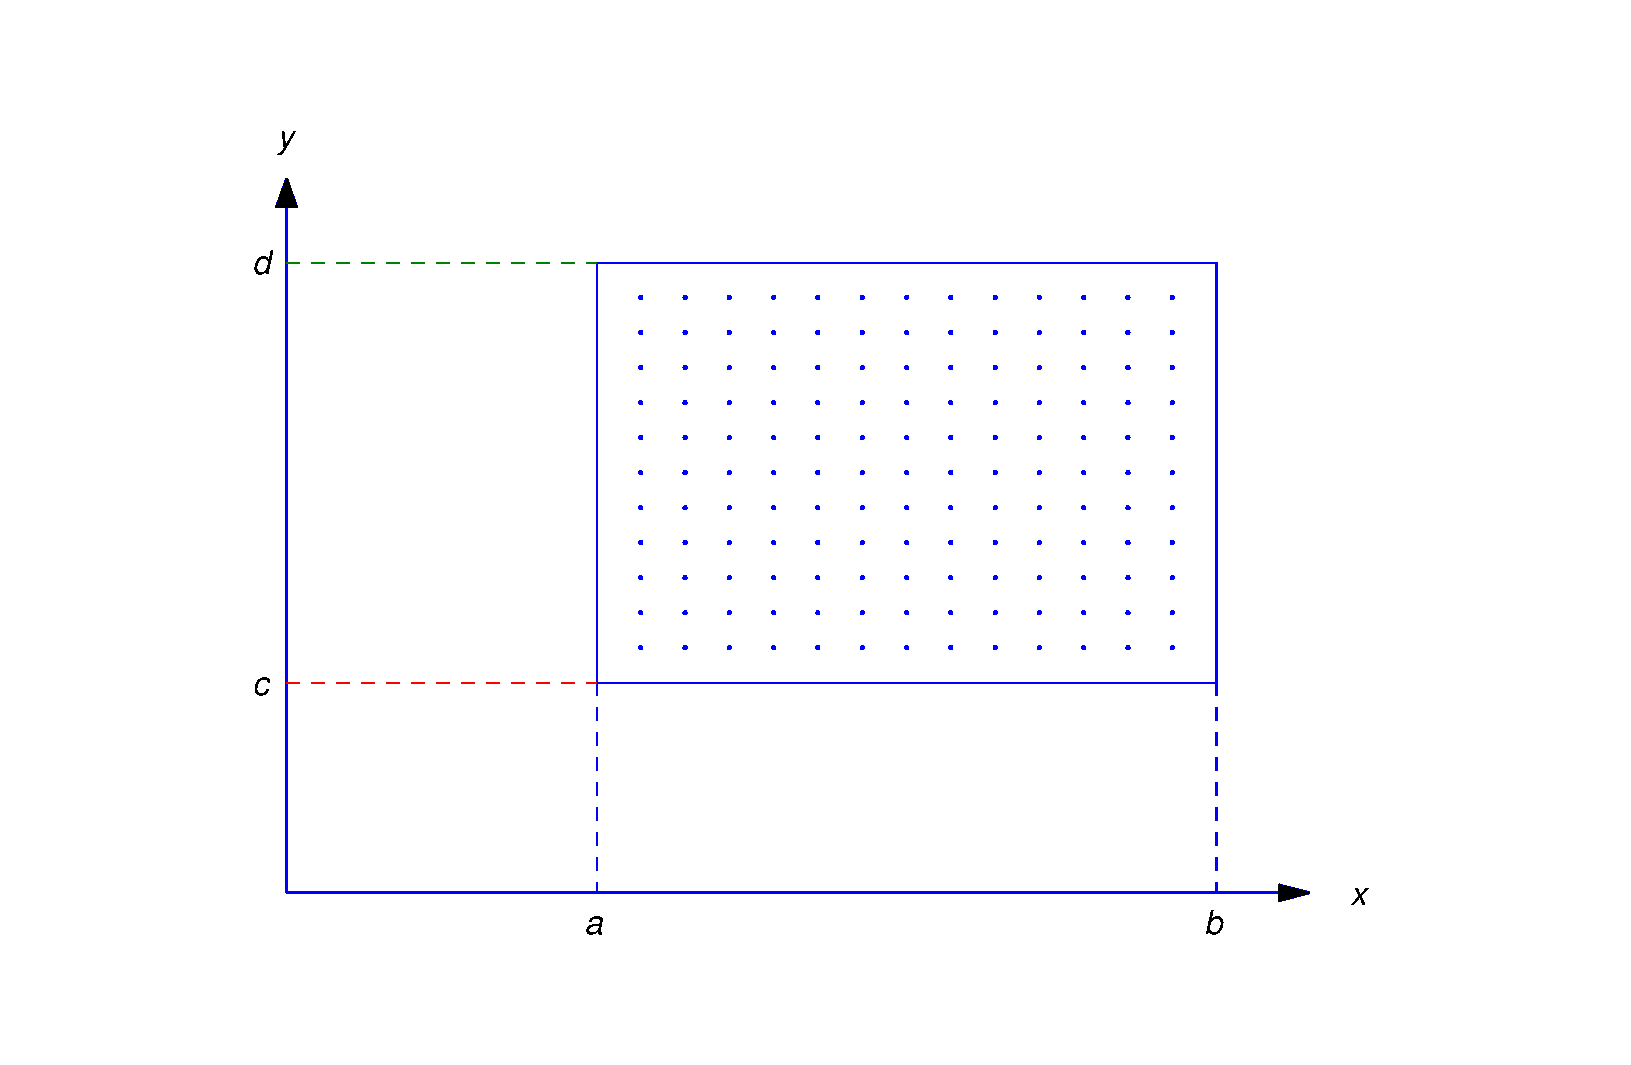
\includegraphics[width = 0.7\textwidth]{fig010301}
\color{blue}
  \caption{\quad  A rectangular grid}
  \label{figure:1.3.1}
\end{figure}

Unfortunately, approximating a direction field and graphing integral
curves in this way is too tedious to be done effectively by hand.
However, there is software  for doing this.
As you'll  see, the combination of  direction fields and
 integral curves gives  useful insights into the behavior of
the solutions of the differential equation even if
we can't obtain exact solutions.

We'll  study numerical methods for solving a single first order
equation \eqref{eq:1.3.1} in Chapter~3. These methods can be
used
to plot solution curves of \eqref{eq:1.3.1} in a rectangular region $R$
{\color{blue}\it if $f$ is continuous on\/} $R$. Figures~\ref{figure:1.3.2},
\ref{figure:1.3.3}, and \ref{figure:1.3.4} show direction fields and solution
curves for the differential equations
$$
 y'=\frac{x^{2}-y^{2}}{1+x^{2}+y^{2}},\quad
y'=1+xy^{2},\text{\quad and \quad}
 y'=\frac{x-y}{1+x^{2}},
$$
which are all of the form \eqref{eq:1.3.1} with $f$
 continuous for all $(x,y)$.

\begin{figure}[htbp]
\color{blue}
  \begin{minipage}[b]{0.5\linewidth}
    \centering
   \scalebox{.6}{
  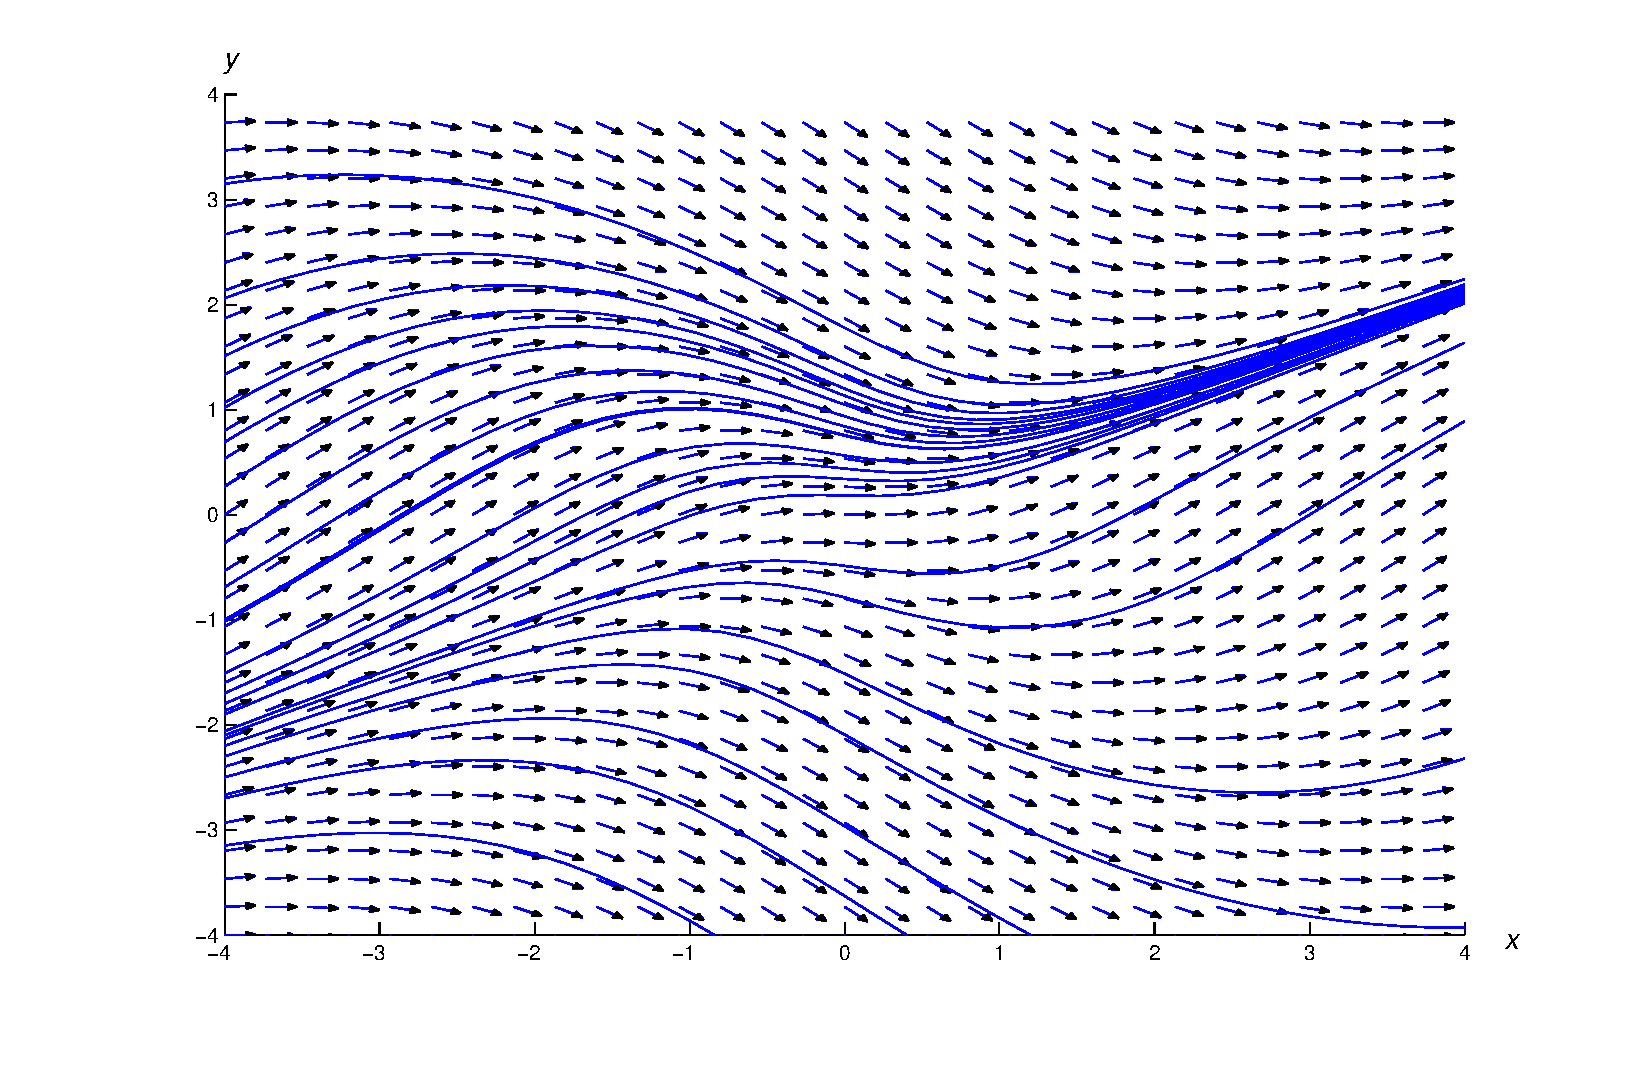
\includegraphics[bb=-78 148 689 643,width=5.67in,height=3.66in,keepaspectratio]{fig010302}}
  \caption{\,A direction field and integral curves for
$y=\dst{\frac{x^{2}-y^{2}}{1+x^{2}+y^{2}}}$}
  \label{figure:1.3.2}
  \end{minipage}
  \hspace{0.6cm}
  \begin{minipage}[b]{0.5\linewidth}
    \centering
   \scalebox{.7}{
  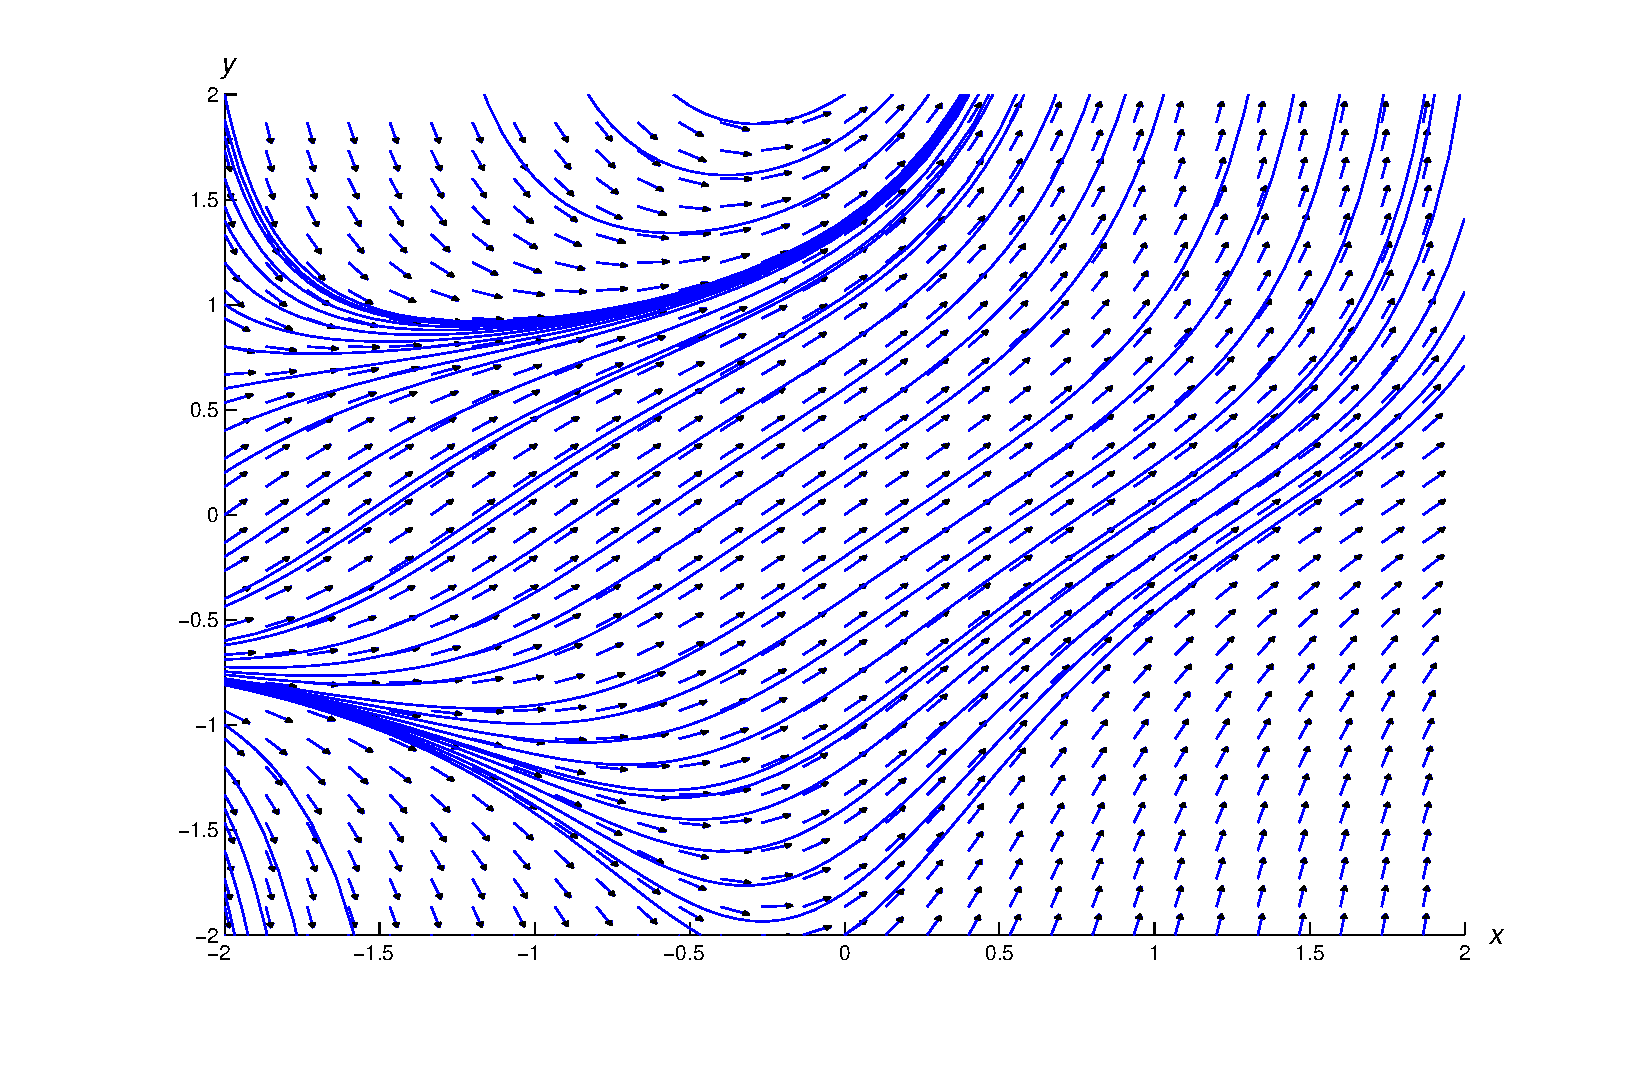
\includegraphics[bb=-78 148 689 643,width=5.67in,height=3.66in,keepaspectratio]{fig010303}}
\caption{A direction field and integral curves
for $y'=1+xy^{2}$}
  \label{figure:1.3.3}
  \end{minipage}
\end{figure}

\begin{figure}[tbp]
  \centering
  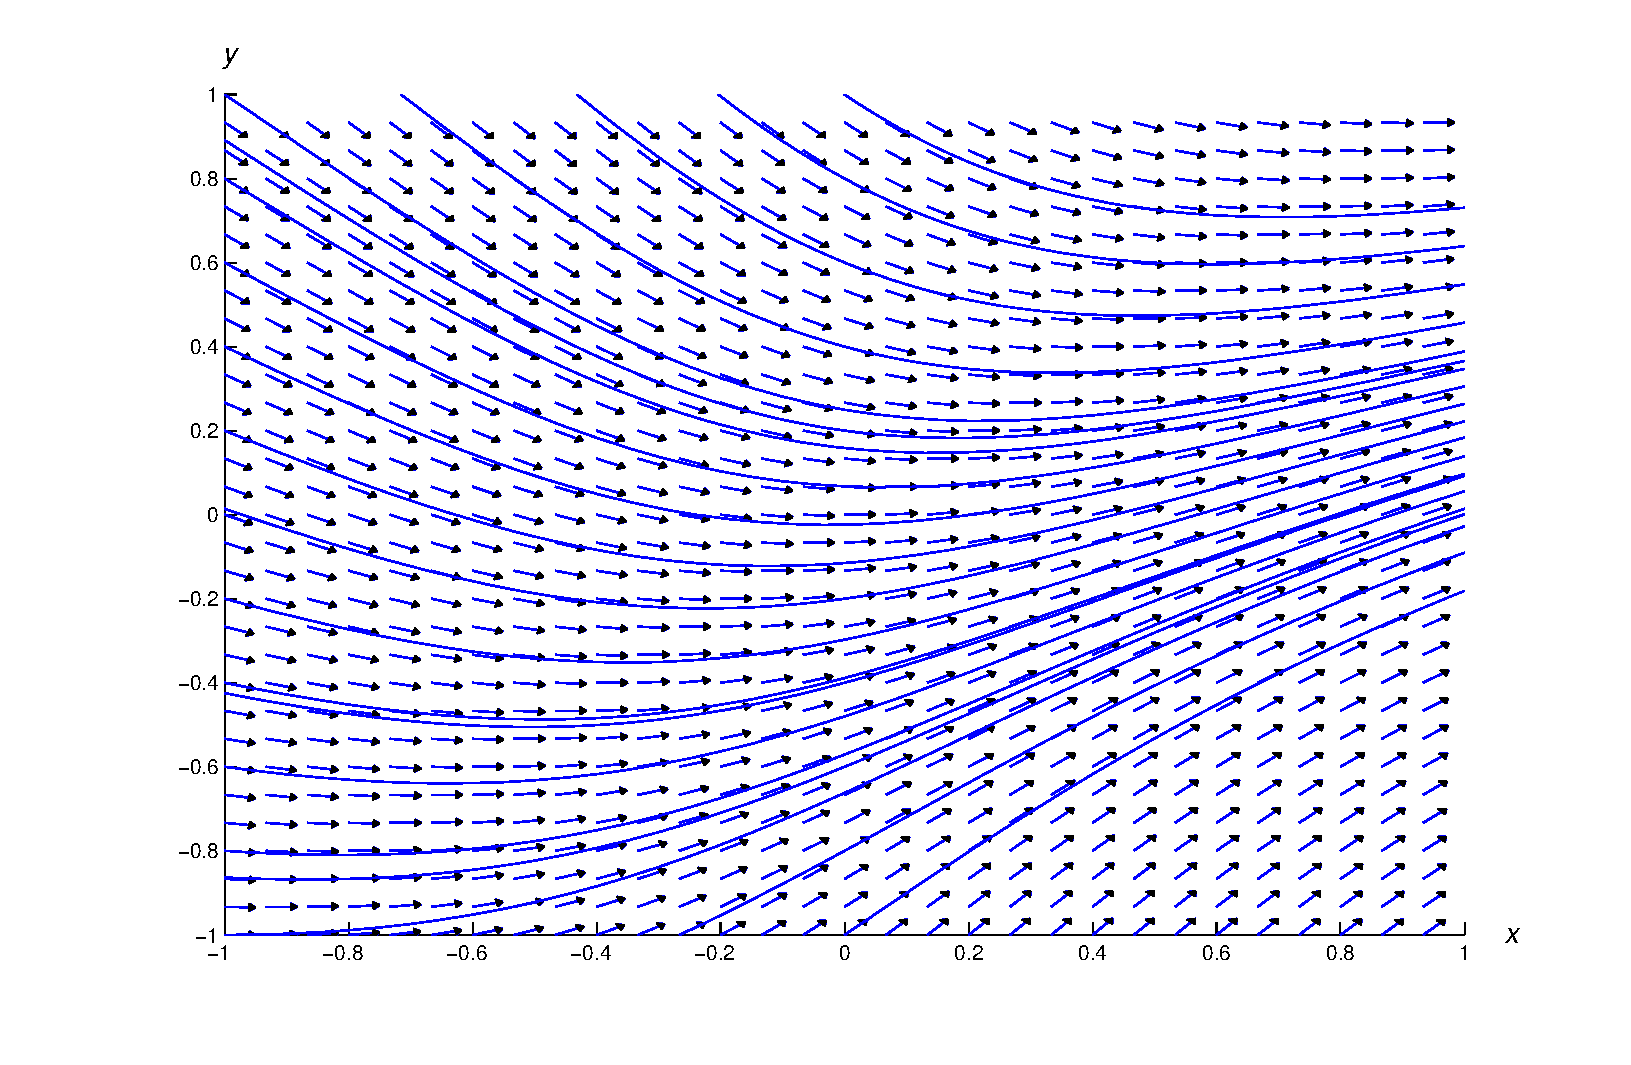
\includegraphics[bb=-78 148 689 643,width=5.67in,height=3.66in,keepaspectratio]{fig010304}
\color{blue}
  \caption{A direction and integral curves for
$y'=\dst{\frac{x-y}{1+x^{2}}}$}
  \label{figure:1.3.4}
\end{figure}

The methods of Chapter~3 won't work for the equation
\begin{equation} \label{eq:1.3.2}
y'=-x/y
\end{equation}
if $R$ contains part of the $x$-axis, since $f(x,y)=-x/y$ is undefined
when $y=0$. Similarly, they won't work for the equation
\begin{equation} \label{eq:1.3.3}
y'=\frac{x^{2}}{1-x^{2}-y^{2}}
\end{equation}
if $R$ contains any part of the unit circle $x^{2}+y^{2}=1$, because the
right side of \eqref{eq:1.3.3} is undefined if $x^{2}+y^{2}=1$. However,
\eqref{eq:1.3.2} and \eqref{eq:1.3.3} can written as
\begin{equation} \label{eq:1.3.4}
y'=\frac{A(x,y)}{B(x,y)}
\end{equation}
where $A$ and $B$ are  continuous on any rectangle $R$. Because of
this,
some differential equation software is based on
numerically solving pairs of equations of the form
\begin{equation} \label{eq:1.3.5}
\frac{dx}{dt}=B(x,y),\quad\frac{dy}{dt}=A(x,y)
\end{equation}
where $x$ and $y$ are regarded as functions of a parameter $t$.
If $x=x(t)$ and $y=y(t)$  satisfy these equations, then
$$
y'=\frac{dy}{dx}=\frac{dy}{dt}\left/\frac{dx}{dt}\right.=\frac{A(x,y)}{B(x,y)},
$$
so $y=y(x)$ satisfies \eqref{eq:1.3.4}.

Eqns.~\eqref{eq:1.3.2} and \eqref{eq:1.3.3} can be reformulated as in
\eqref{eq:1.3.4} with
$$
\frac{dx}{dt}=-y,\quad\frac{dy}{dt}=x
$$
and
$$
\frac{dx}{dt}=1-x^{2}-y^{2},\quad\frac{dy}{dt}=x^{2},
$$
respectively. Even if $f$ is continuous and otherwise ``nice''
throughout $R$, your software  may require you to
reformulate the equation $y'=f(x,y)$ as
$$
\frac{dx}{dt}=1,\quad\frac{dy}{dt}=f(x,y),
$$
which is of the form \eqref{eq:1.3.5} with $A(x,y)=f(x,y)$ and
$B(x,y)=1$.

Figure~\ref{figure:1.3.5} shows a direction field and some integral curves
for \eqref{eq:1.3.2}. As we saw in
Example~\ref{example:1.2.1} and will verify
again in Section~2.2, the integral curves of \eqref{eq:1.3.2}
are circles centered at the origin.

\begin{figure}[H]
  \centering
  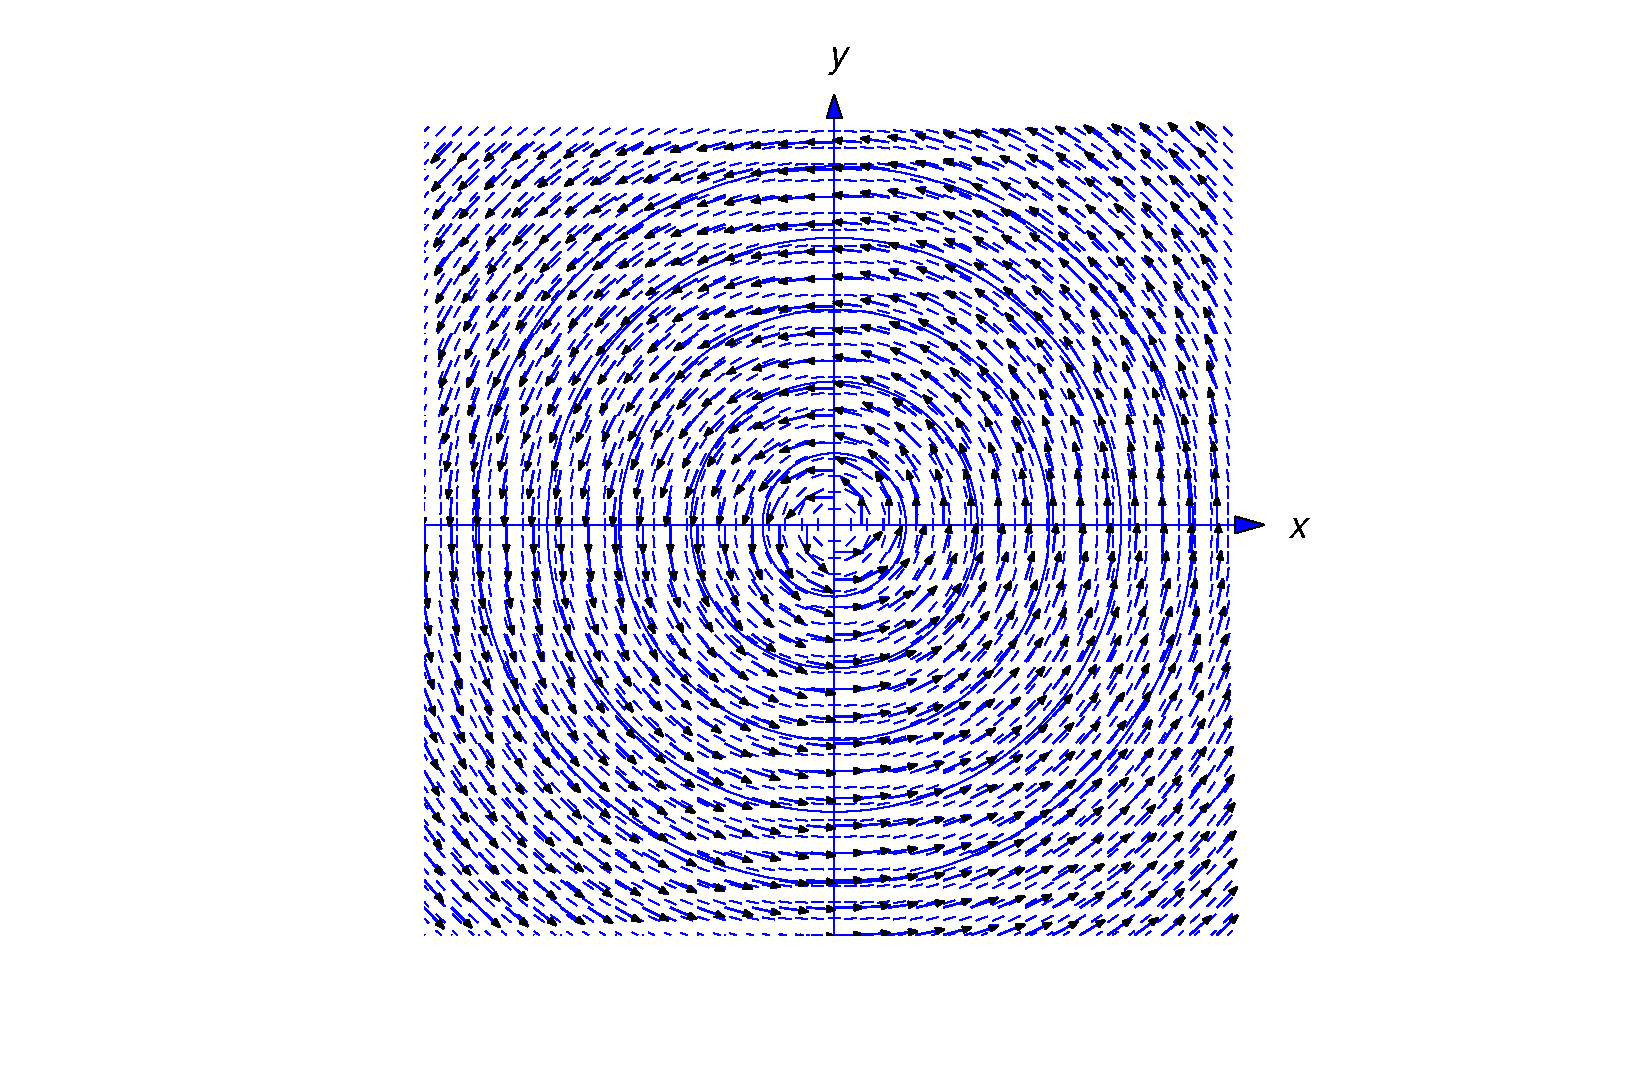
\includegraphics[bb=-78 148 689 643,width=5.67in,height=3.66in,keepaspectratio]{fig010305}
\color{blue}
\caption{A direction field and integral curves for
$y'=-\dst\frac{x}{y}$}
  \label{figure:1.3.5}
\end{figure}

Figure~\ref{figure:1.3.6} shows a direction field and some integral curves
for \eqref{eq:1.3.3}. The integral curves near the top and bottom are
solution curves. However, the integral curves near the middle are more
complicated. For example, Figure~\ref{figure:1.3.7} shows the integral
curve through the origin. The vertices of the dashed rectangle are on
the circle $x^{2}+y^{2}=1$ ($a\approx.846$, $b\approx.533$), where all
integral curves of \eqref{eq:1.3.3} have infinite slope. There are
three solution curves of \eqref{eq:1.3.3} on the integral curve in the
figure: the segment above the level $y=b$ is the graph of a solution
on $(-\infty,a)$, the segment below the level $y=-b$ is the graph of a
solution on $(-a,\infty)$, and the segment between these two levels is
the graph of a solution on $(-a,a)$.

\technology
 \medskip
As you study from this book, you'll often be asked to use
computer software and graphics. Exercises with this intent are marked
as \Cex\, (computer or calculator required), \CGex\, (computer and/or
graphics required), or \Lex\ (laboratory work requiring software
and/or graphics).
 Often
you may not completely understand how the software does what it does.
This is similar to the situation most people are in when they drive
automobiles or watch television, and it doesn't decrease the value
of using modern technology as an aid to learning. Just be careful that
you use the technology as a supplement to thought rather than a
substitute for it.

\begin{figure}[htbp]
\color{blue}
  \begin{minipage}[b]{0.5\linewidth}
    \centering
   \scalebox{.7}{
  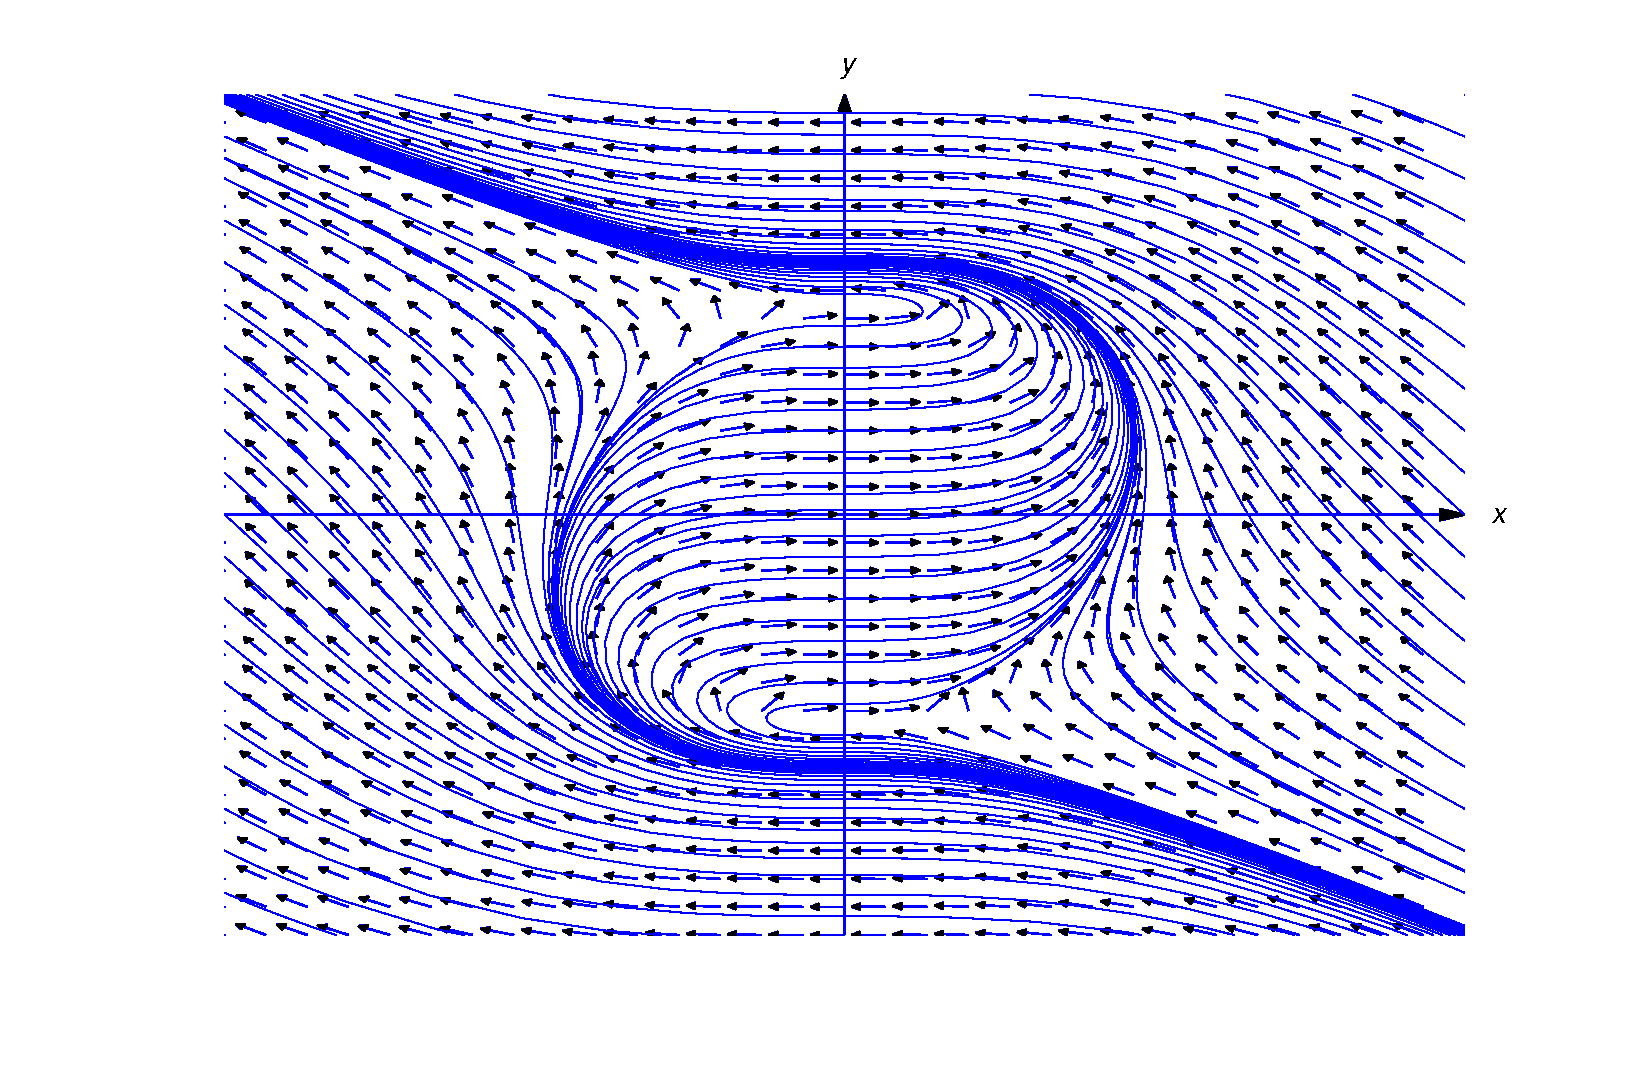
\includegraphics[bb=-78 148 689 643,width=5.67in,height=3.66in,keepaspectratio]{fig010306} }
\caption{A direction field and integral curves for
$y'=\dst\frac{x^{2}}{1-x^{2}-y^{2}}$}
  \label{figure:1.3.6}
  \end{minipage}
  \hspace{0.6cm}
  \begin{minipage}[b]{0.5\linewidth}
    \centering
   \scalebox{.7}{
  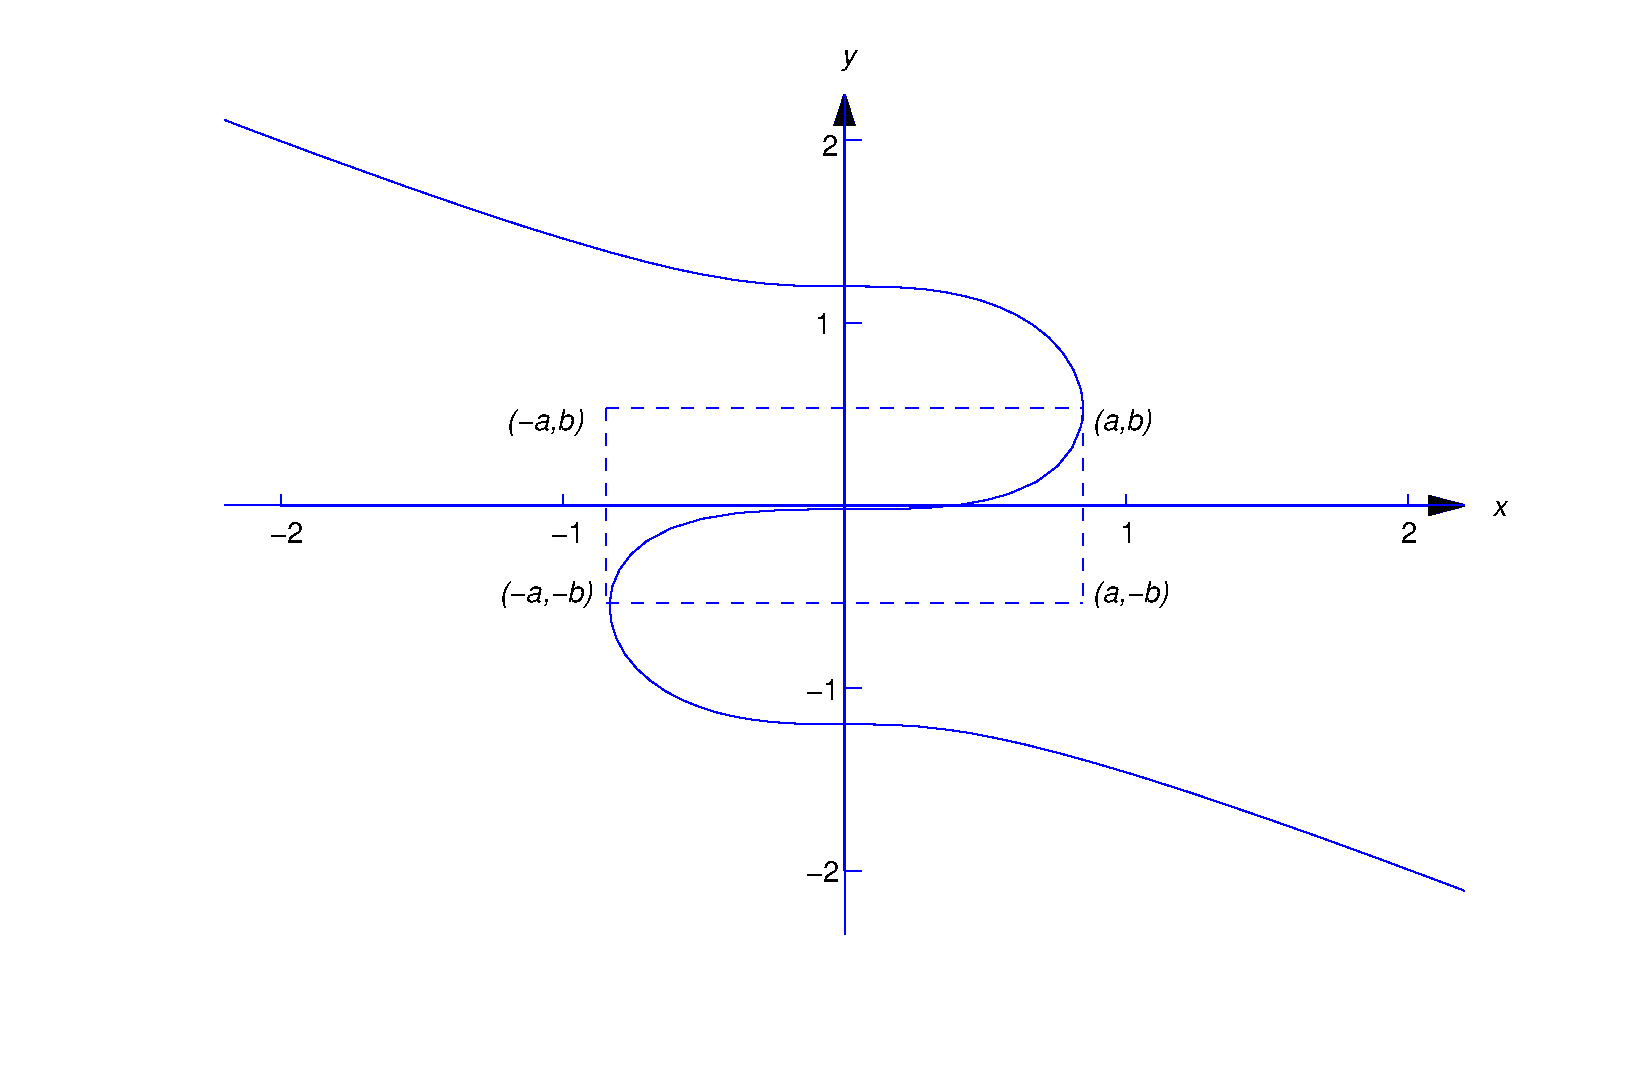
\includegraphics[bb=-78 148 689 643,width=5.67in,height=3.66in,keepaspectratio]{fig010307} }
\caption{}
  \label{figure:1.3.7}
  \end{minipage}
\end{figure}

\enlargethispage{1in}

\exercises
\noindent
\emph{In Exercises~{\color{red}\rm\bf 1--11} a  direction
field is drawn for the given equation. Sketch some integral curves.}

\begin{figure}[H]
  \color{blue}
  \centering
  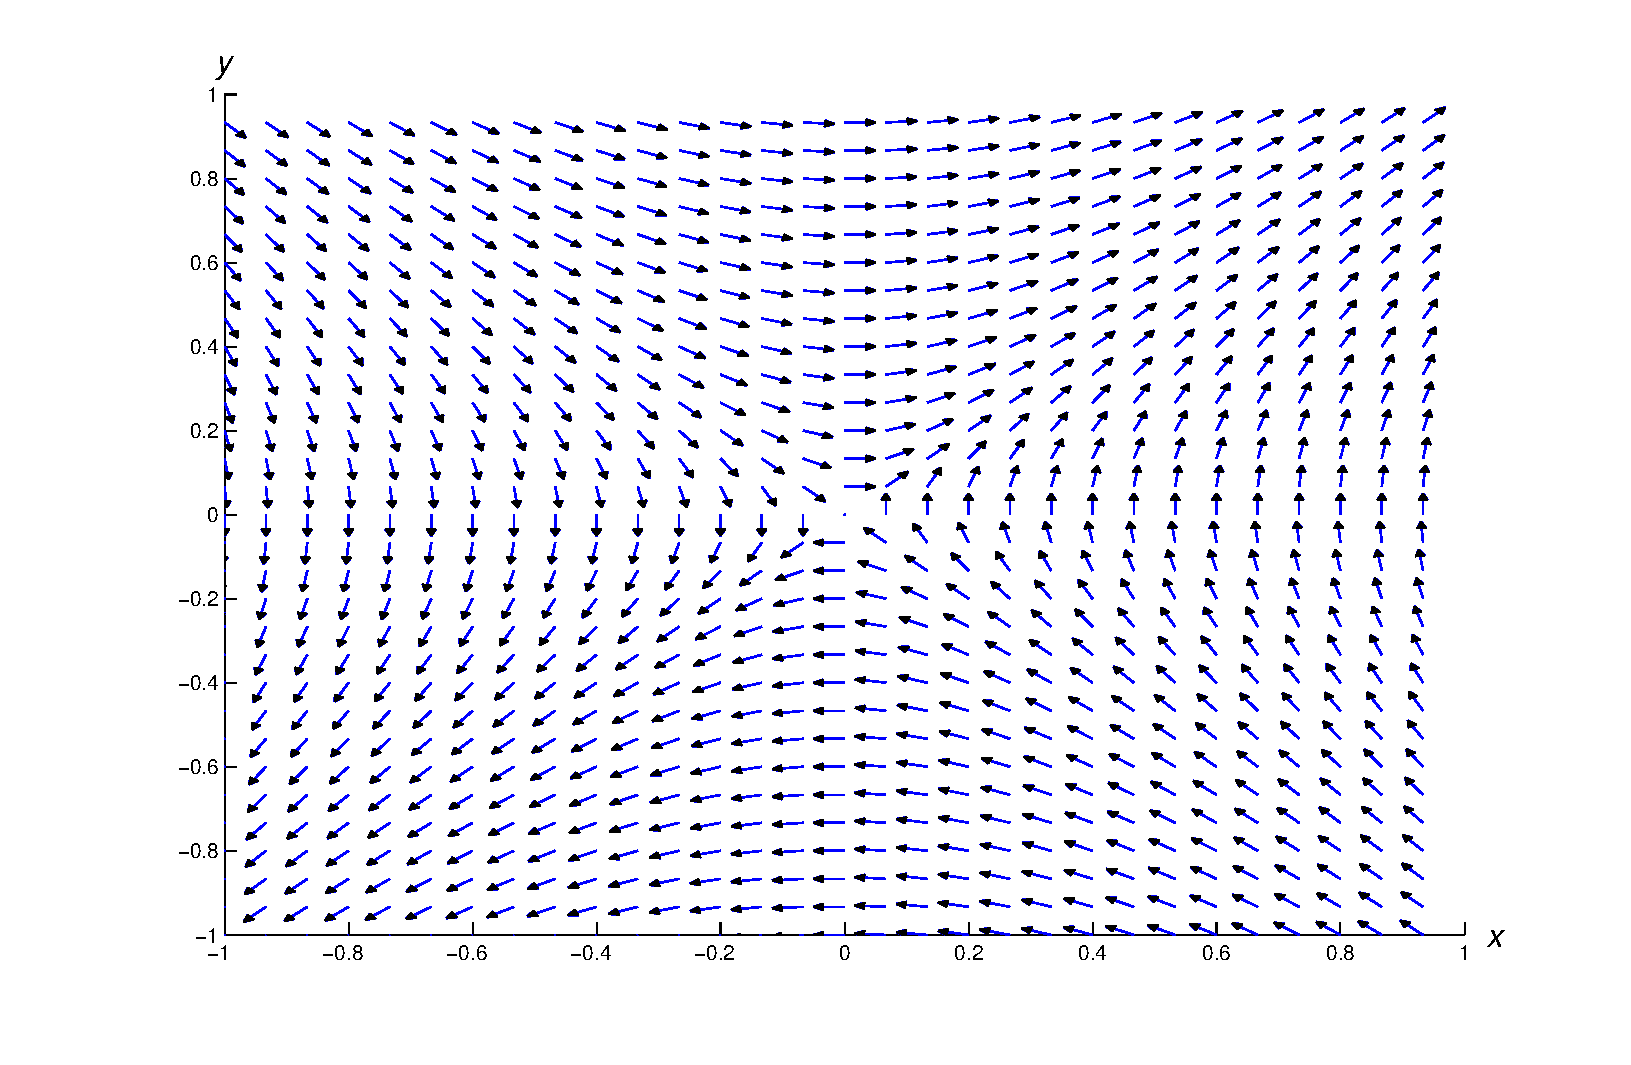
\includegraphics[bb=-78 148 689 643,width=5.67in,height=3.66in,keepaspectratio]{exer010301}
  \caption*{{\color{red}\bf 1}\; A direction field for
$y'=\dst{\frac{x}{y}}$}
\end{figure}

\newpage

\begin{figure}[H]
  \color{blue}
  \centering
  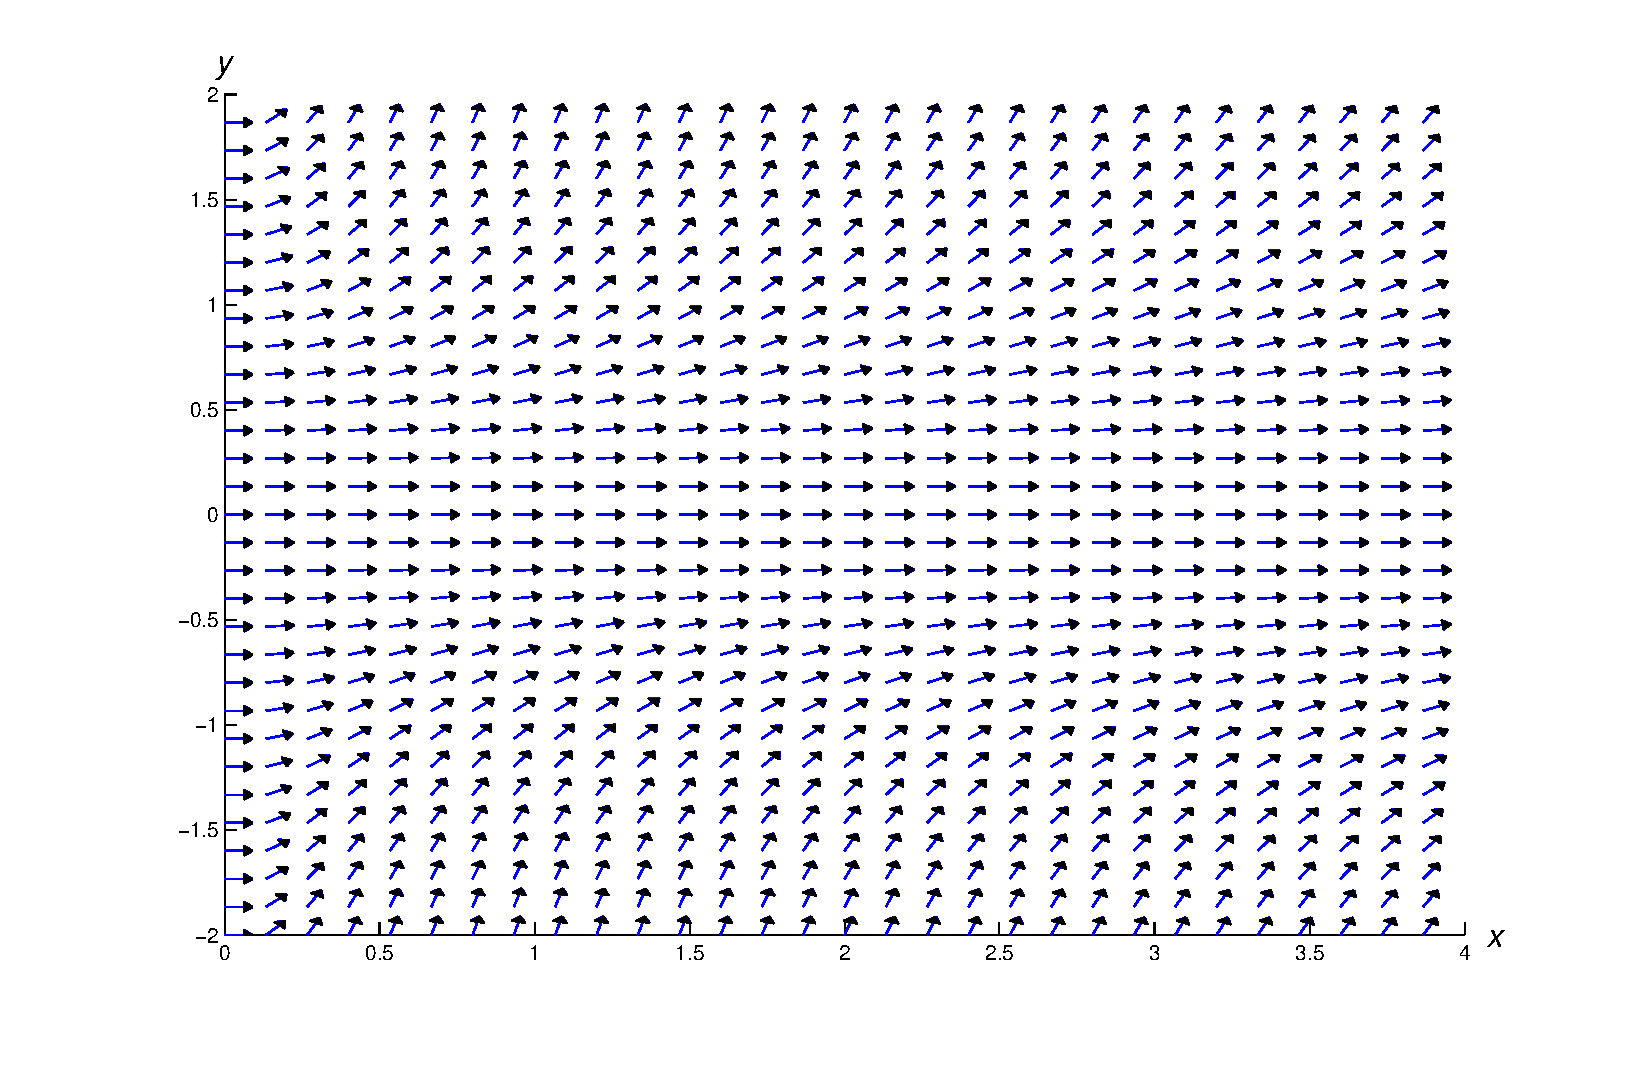
\includegraphics[bb=-78 148 689 643,width=5.67in,height=3.66in,keepaspectratio]{exer010302}
  \caption*{{\color{red}\bf 2}\; A direction field for
 $\dst{y'=\dst\frac{2xy^{2}}{1+x^{2}}}$\quad}
\end{figure}

\begin{figure}[H]
  \color{blue}
  \centering
  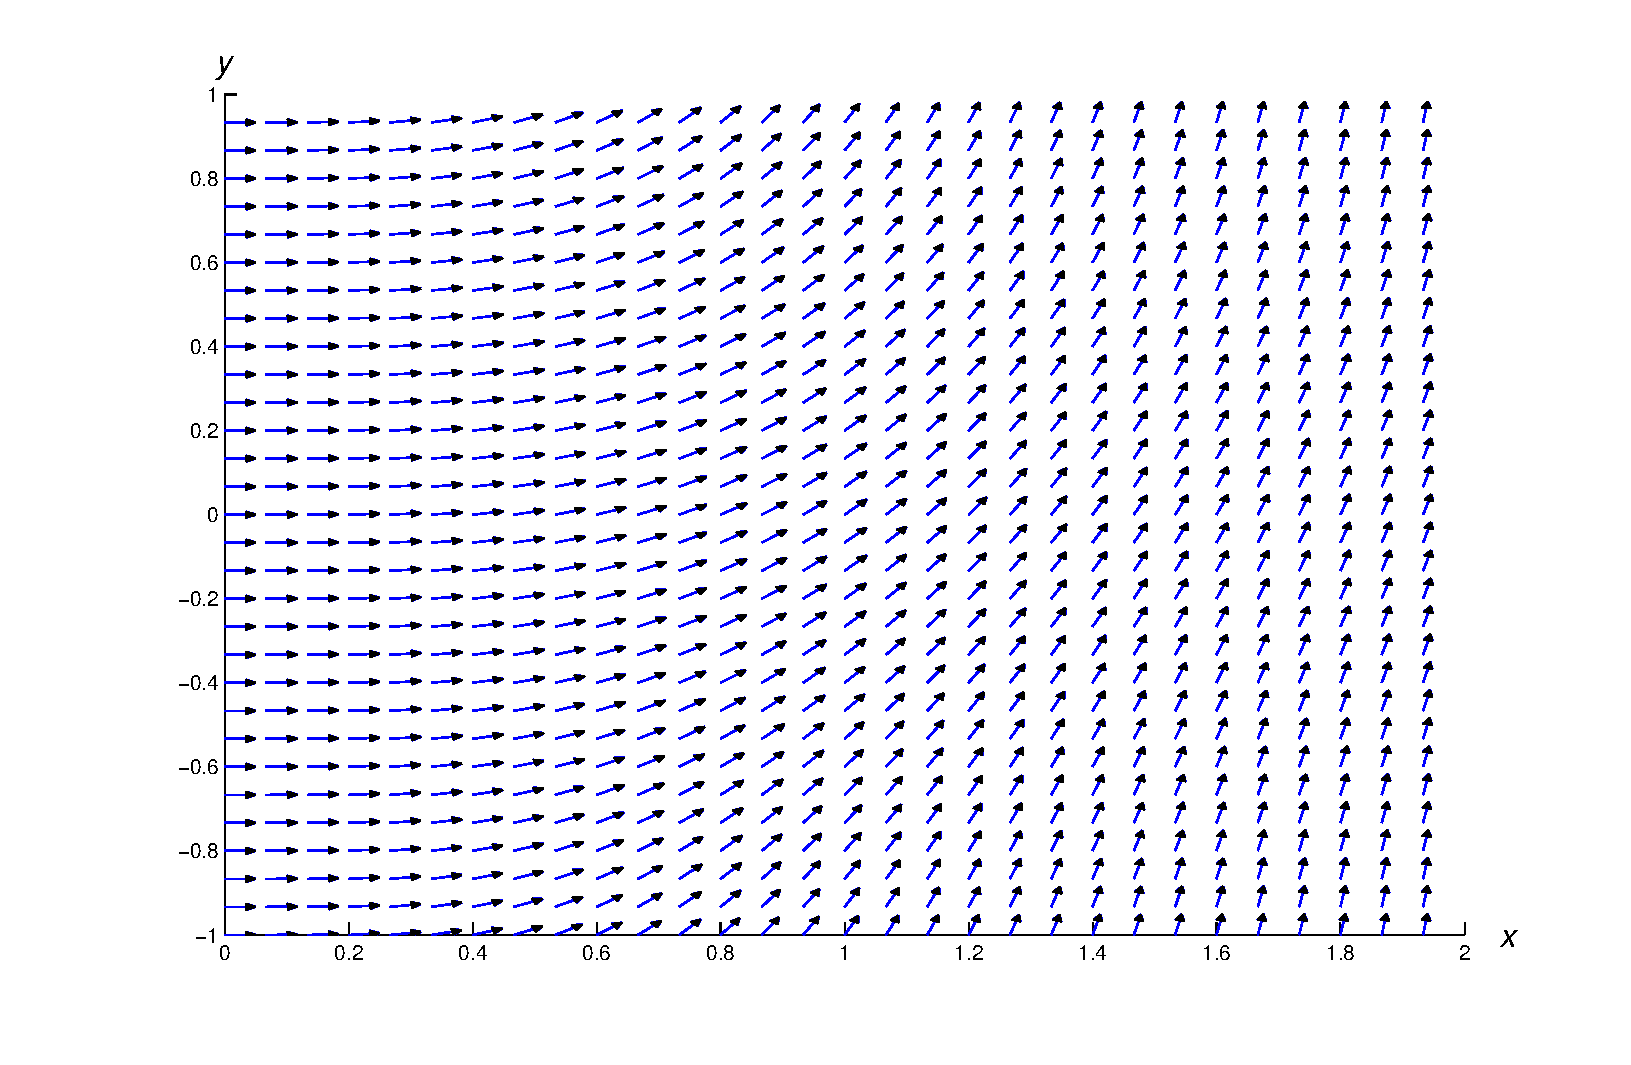
\includegraphics[bb=-78 148 689 643,width=5.67in,height=3.66in,keepaspectratio]{exer010303}
  \caption*{{\color{red}\bf 3}\; A direction field for
 $y'=x^{2}(1+y^{2})$}
\end{figure}

\begin{figure}[H]
  \color{blue}
  \centering
  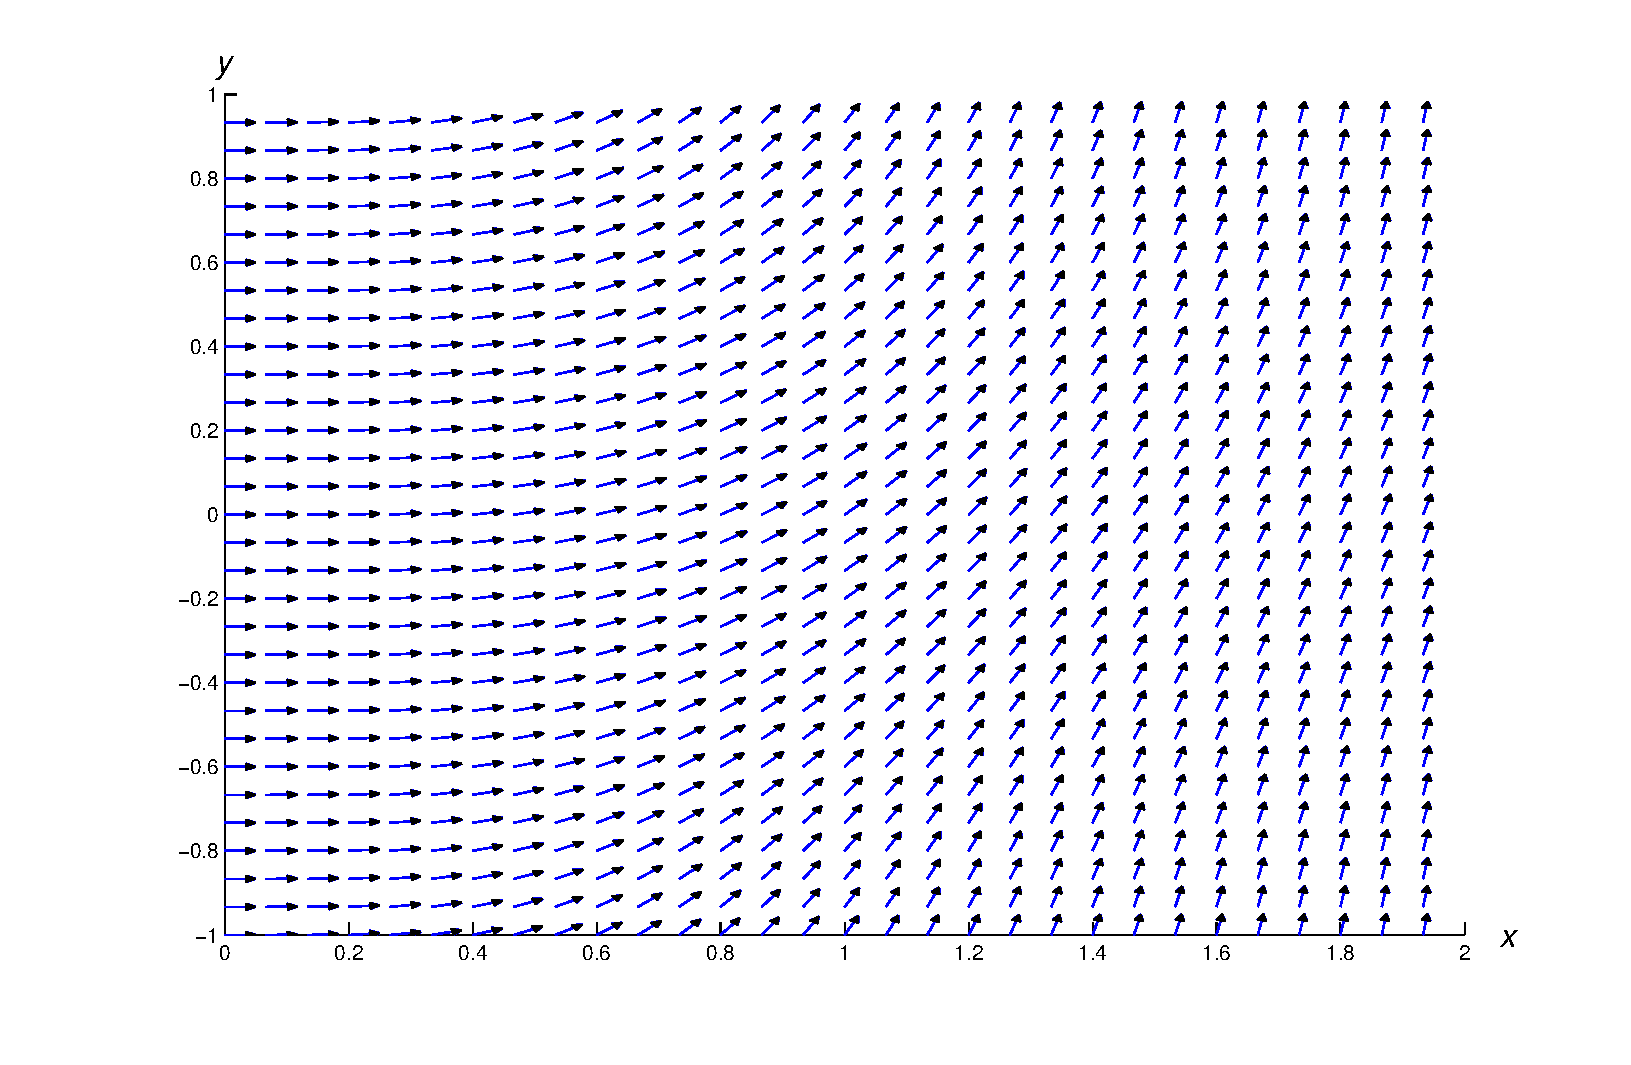
\includegraphics[bb=-78 148 689 643,width=5.67in,height=3.66in,keepaspectratio]{exer010304}
  \caption*{{\color{red}\bf 4}\; A direction field for
$y'=\dst\frac{1}{1+x^{2}+y^{2}}$}
\end{figure}

\begin{figure}[H]
  \color{blue}
  \centering
  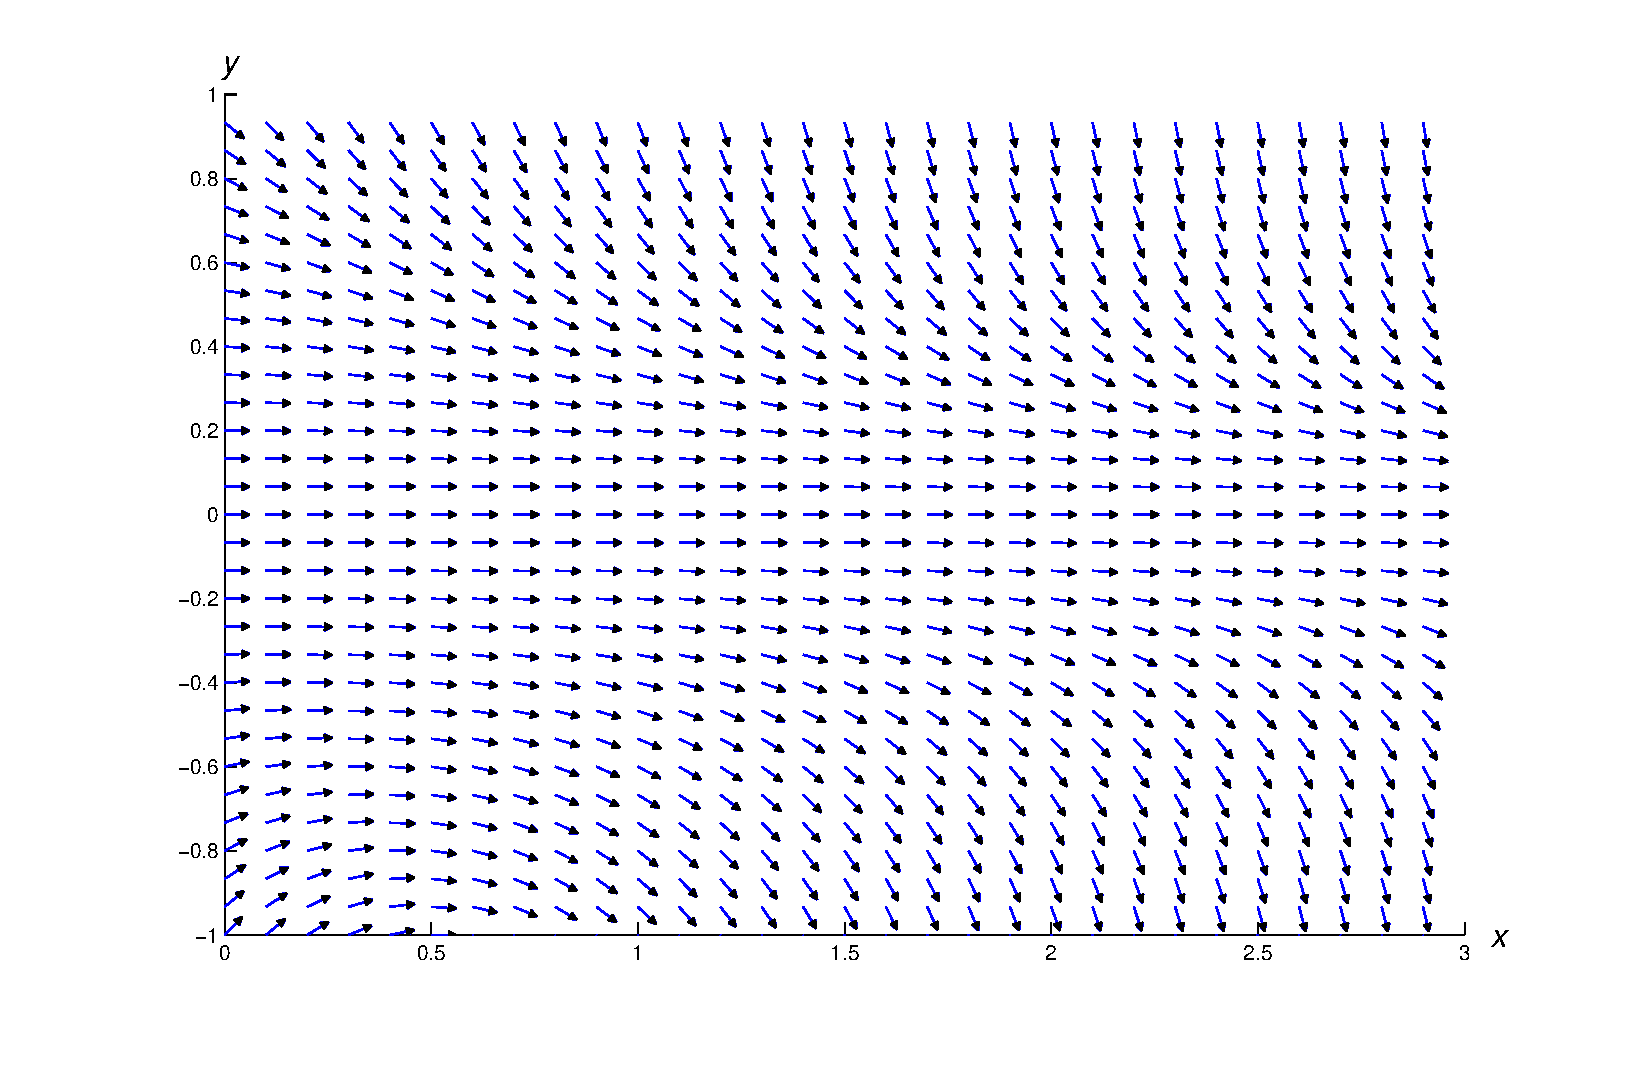
\includegraphics[bb=-78 148 689 643,width=5.67in,height=3.66in,keepaspectratio]{exer010305}
  \caption*{{\color{red}\bf 5}\; A direction field for
$y'=-(2xy^{2}+y^{3})$}
\end{figure}

\begin{figure}[H]
  \color{blue}
  \centering
  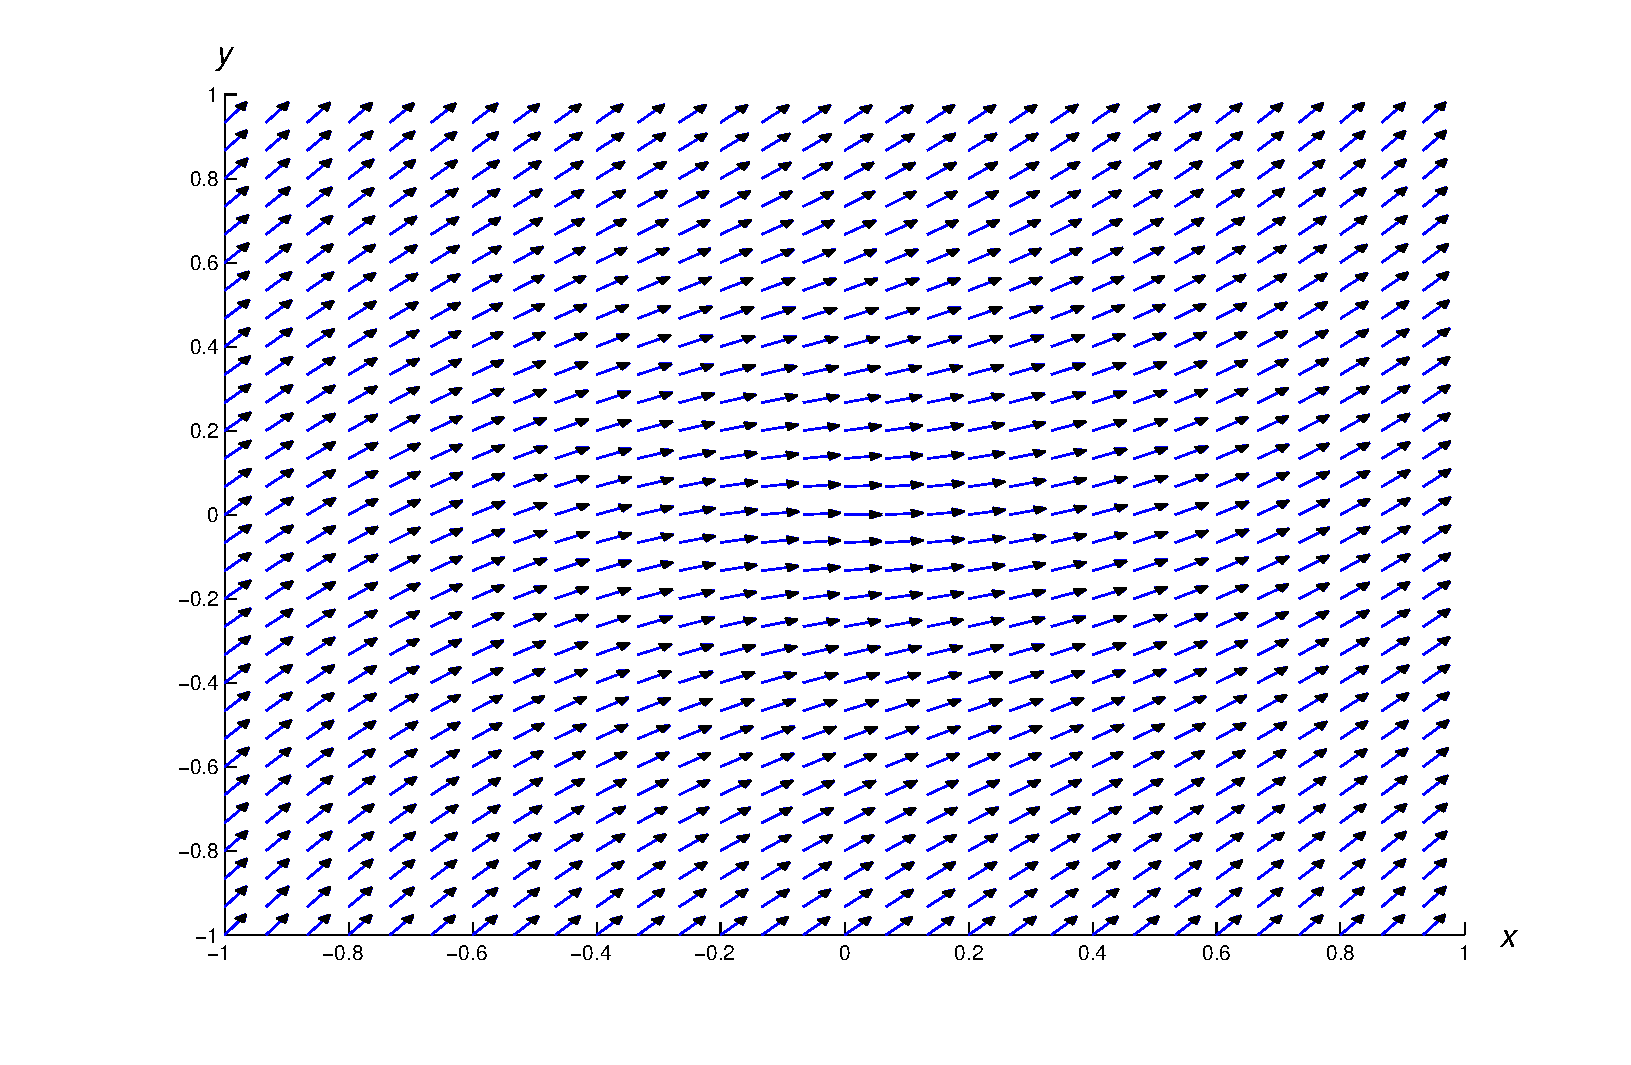
\includegraphics[bb=-78 148 689 643,width=5.67in,height=3.66in,keepaspectratio]{exer010306}
  \caption*{{\color{red}\bf 6}\; A direction field for
$y'=(x^{2}+y^{2})^{1/2}$}
\end{figure}

\begin{figure}[H]
  \color{blue}
  \centering
  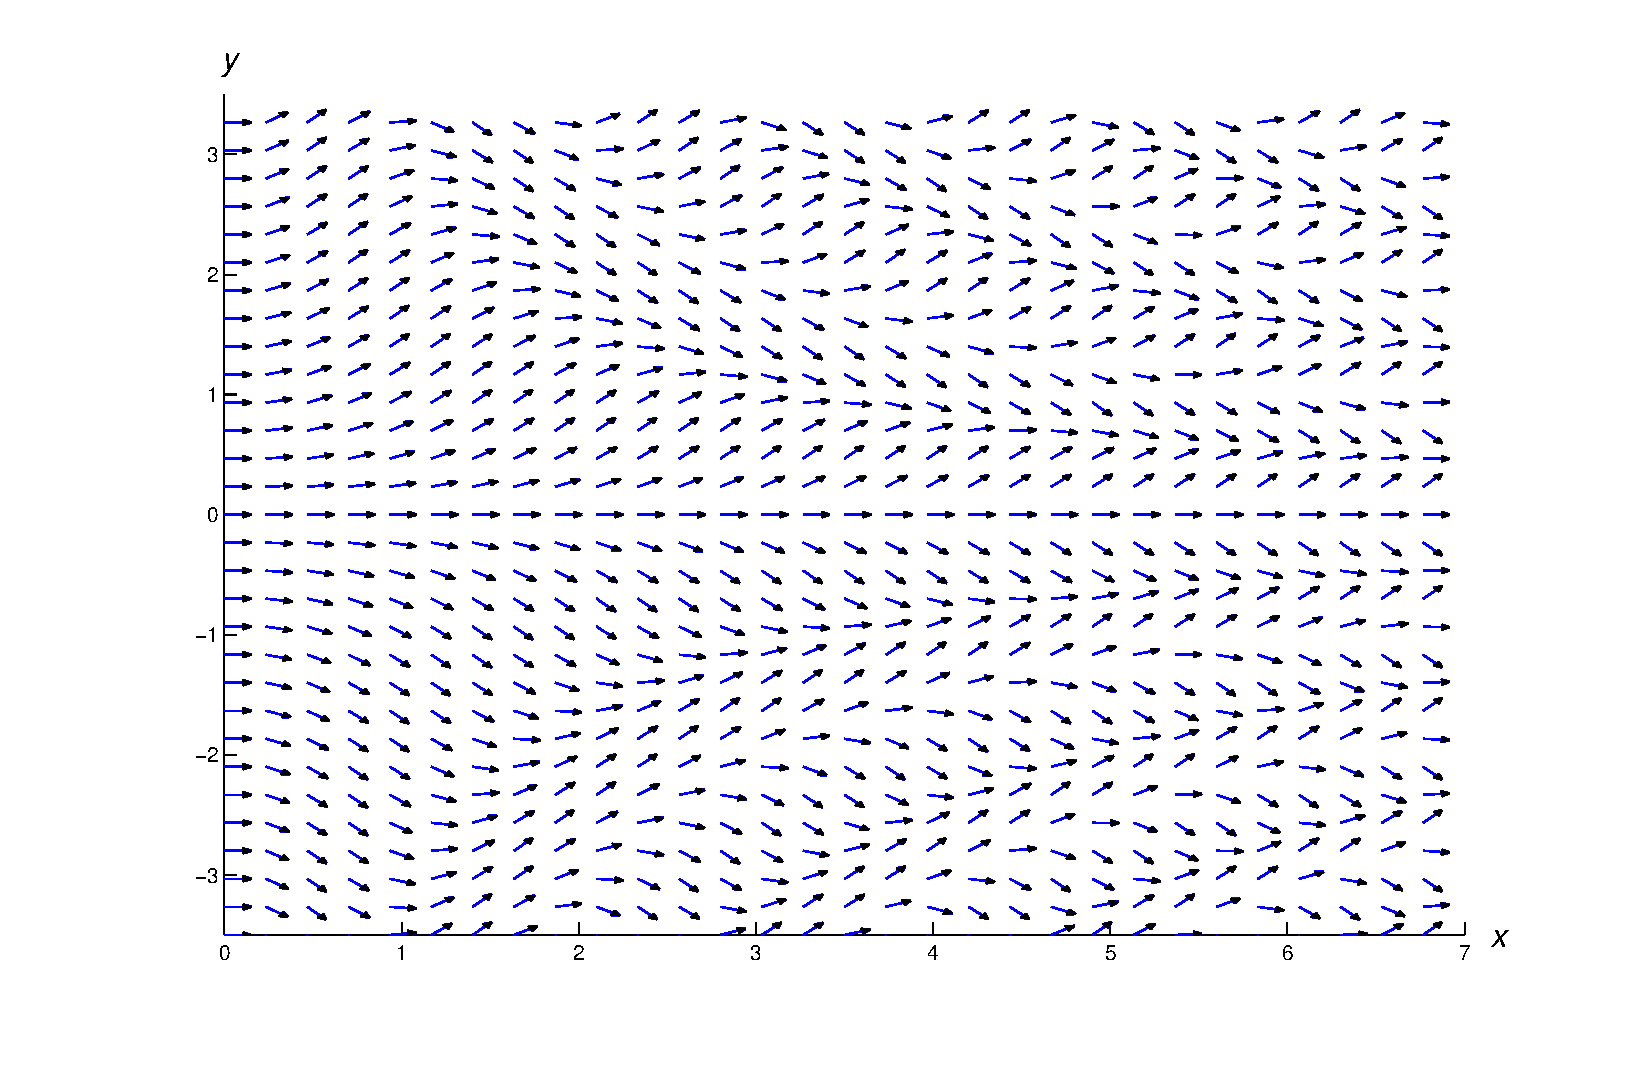
\includegraphics[bb=-78 148 689 643,width=5.67in,height=3.66in,keepaspectratio]{exer010307}
  \caption*{{\color{red}\bf 7}\; A direction field for
$y'=\sin xy$}
\end{figure}

\begin{figure}[H]
  \color{blue}
  \centering
  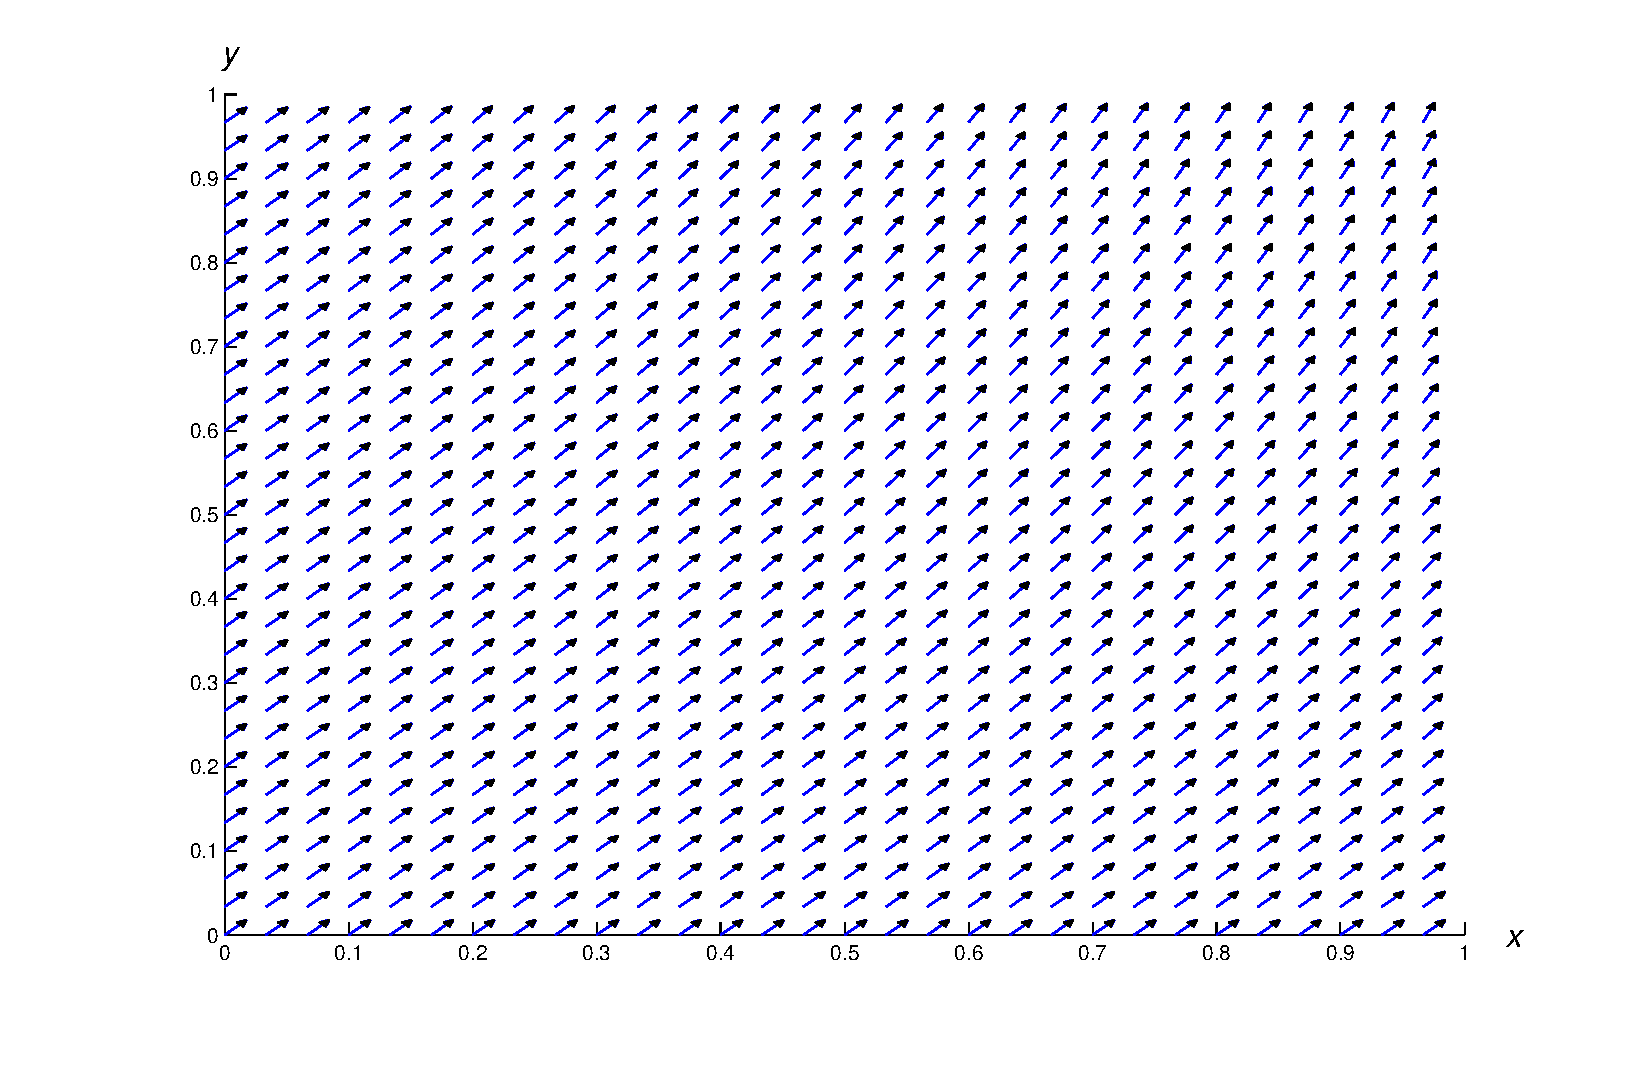
\includegraphics[bb=-78 148 689 643,width=5.67in,height=3.66in,keepaspectratio]{exer010308}
  \caption*{{\color{red}\bf 8}\; A direction field for
 $y'=e^{xy}$}
\end{figure}

\begin{figure}[H]
  \color{blue}
  \centering
  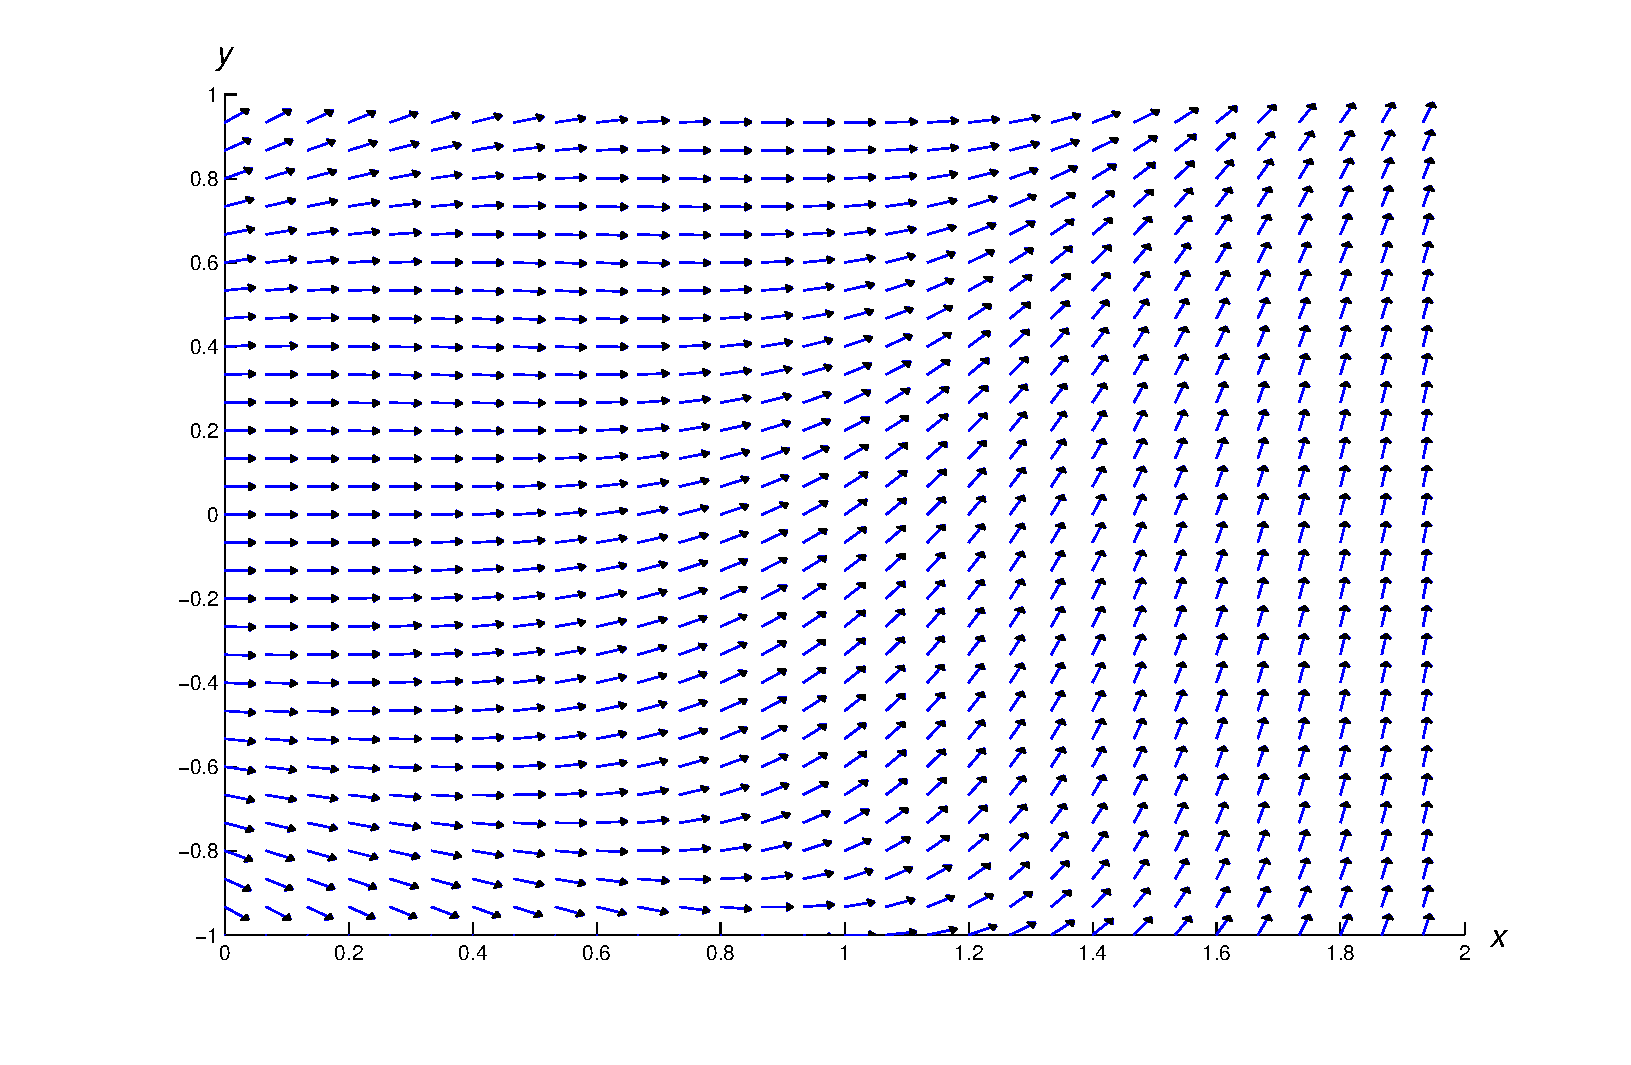
\includegraphics[bb=-78 148 689 643,width=5.67in,height=3.66in,keepaspectratio]{exer010309}
  \caption*{{\color{red}\bf 9}\; A direction field for
$y'=(x-y^{2})(x^{2}-y)$}
\end{figure}

\begin{figure}[H]
  \color{blue}
  \centering
  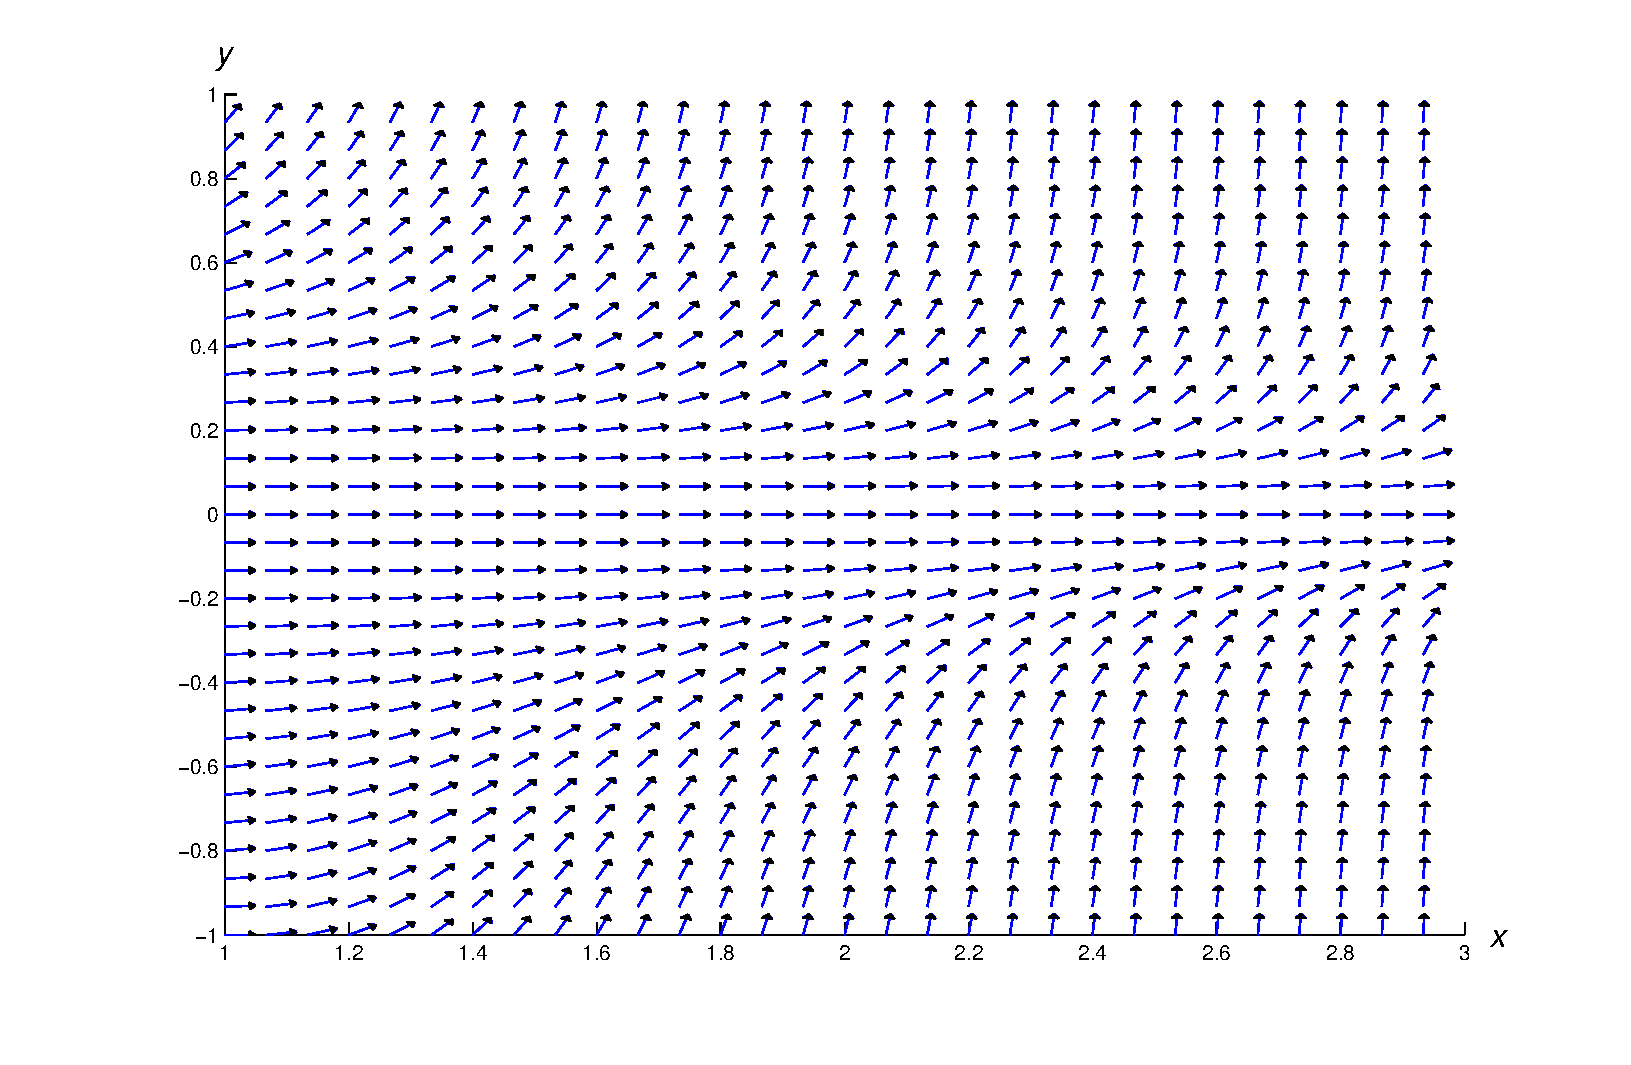
\includegraphics[bb=-78 148 689 643,width=5.67in,height=3.66in,keepaspectratio]{exer010310}
  \caption*{{\color{red}\bf 10}\; A direction field for
$y'=x^{3}y^{2}+xy^{3}$}
\end{figure}

\begin{figure}[H]
  \color{blue}
  \centering
  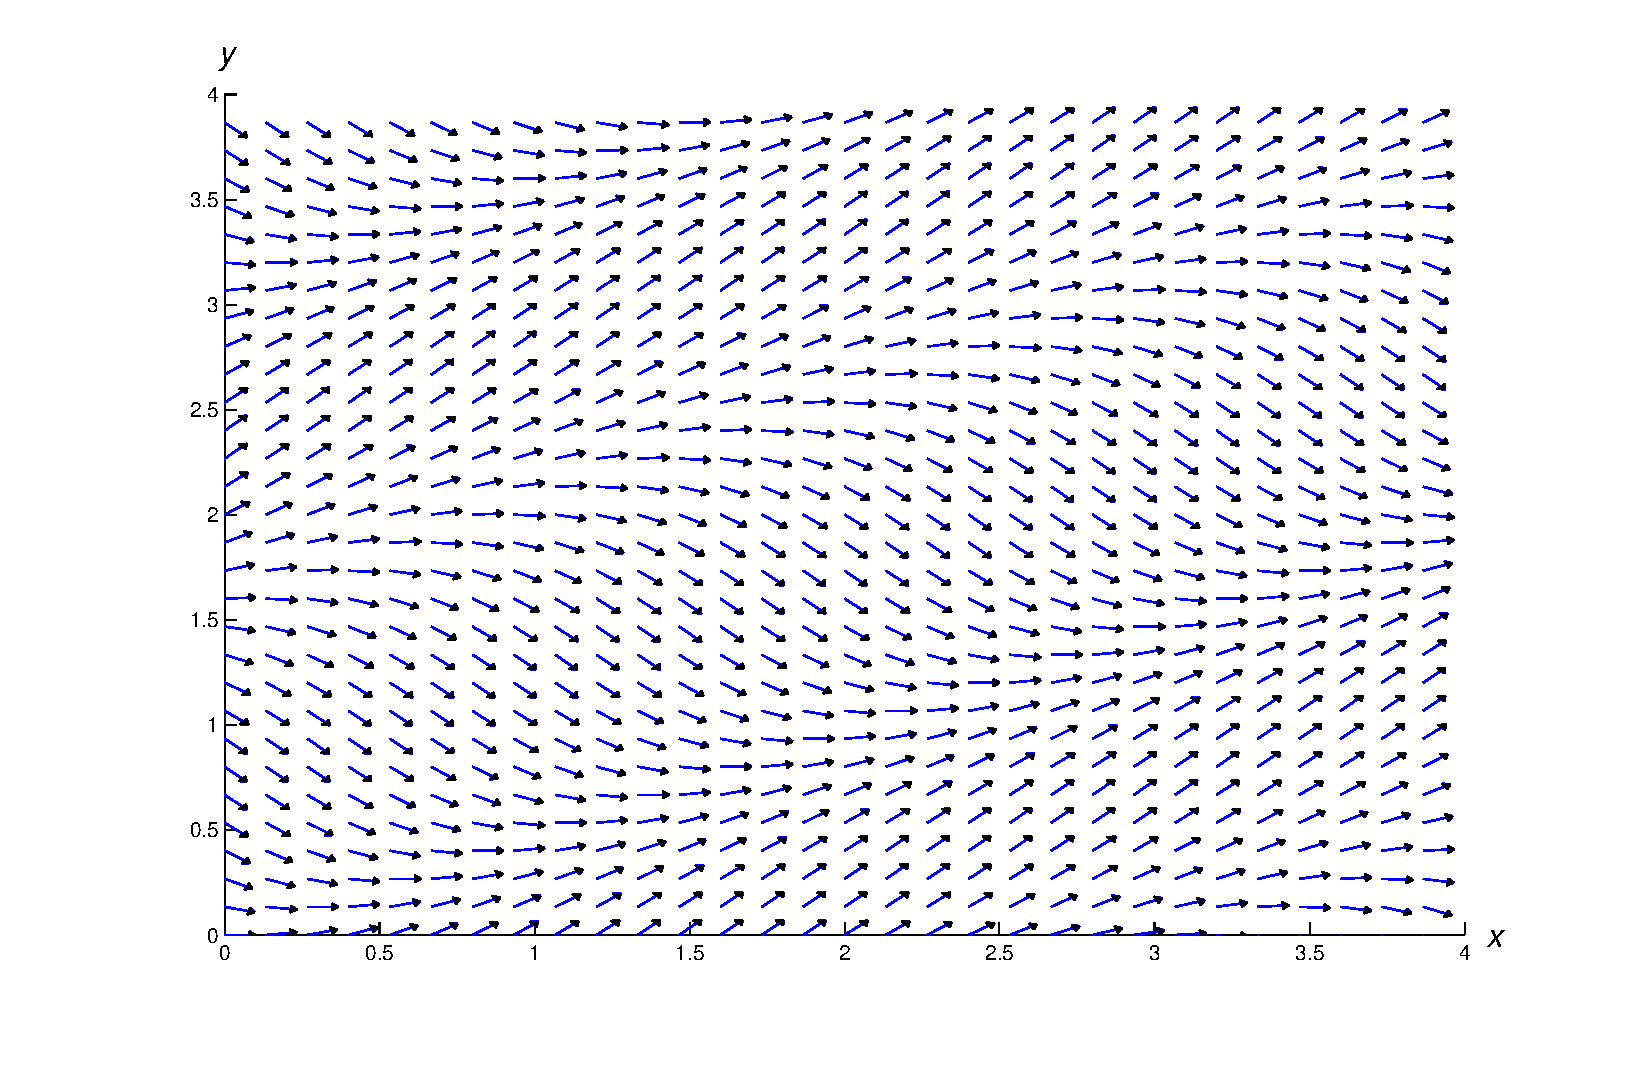
\includegraphics[bb=-78 148 689 643,width=5.67in,height=3.66in,keepaspectratio]{exer010311}
  \caption*{{\color{red}\bf 11}\; A direction field for
$y'=\sin(x-2y)$}
\end{figure}

\newpage
\emph{In Exercises~\ref{exer:1.3.12}-\ref{exer:1.3.22} construct a
direction
field and plot some integral curves in the indicated rectangular region.}

\begin{exerciselist}[start=12]
\item\label{exer:1.3.12}\CGex
$y'=y(y-1);\quad\{-1\le x\le2,\ -2\le y\le2\}$

\item\label{exer:1.3.13} \CGex
$y'=2-3xy;\quad\{-1\le x\le4,\ -4\le y\le4\}$

\item\label{exer:1.3.14} \CGex
$y'=xy(y-1);\quad\{-2\le x\le2,\ -4\le y\le4\}$

\item\label{exer:1.3.15}\CGex
$y'=3x+y;\quad\{-2\le x\le2,\ 0\le y\le4\}$

\item\label{exer:1.3.16} \CGex
$y'=y-x^{3};\quad\{-2\le x\le2,\ -2\le y\le2\}$

\item\label{exer:1.3.17}\CGex
$y'=1-x^{2}-y^{2};\quad\{-2\le x\le2,\ -2\le y\le2\}$

\item\label{exer:1.3.18}\CGex
$y'=x(y^{2}-1);\quad\{-3\le x\le3,\ -3\le y\le2\}$

\item\label{exer:1.3.19}\CGex
$y'=\dst\frac{x}{y(y^{2}-1)};\quad\{-2\le x\le2,\ -2\le y\le2\}$

\item\label{exer:1.3.20}\CGex
$y'=\dst\frac{xy^{2}}{y-1};\quad\{-2\le x\le2,\ -1\le y\le4\}$

\item\label{exer:1.3.21}\CGex
$y'=\dst\frac{x(y^{2}-1)}{y};\quad\{-1\le x\le1,\ -2\le y\le2\}$

\item\label{exer:1.3.22}\CGex
$y'=-\dst\frac{x^{2}+y^{2}}{1-x^{2}-y^{2}};\quad\{-2\le x\le2,\ -2\le y\le2\}$

\item\label{exer:1.3.23} \Lex
By suitably renaming the constants and  dependent variables
in the equations
$$
T'=-k(T-T_{m})
\eqno{\rm(A)}
$$
and
$$
G'=-\lambda G+r
\eqno{\rm(B)}
$$
discussed in Section~1.2 in connection with Newton's
law of cooling and absorption of glucose in the body, we can
write both as
$$
y'=-ay+b,
\eqno{\rm(C)}
$$
where $a$ is a positive constant and $b$ is an arbitrary
constant. Thus, (A) is of the form (C) with $y=T$, $a=k$, and
$b=kT_{m}$, and (B) is of the form (C) with $y=G$,
$a=\lambda$, and $b=r$. We'll encounter equations of the form
(C) in many other applications in Chapter~2.

Choose a positive  $a$  and an
arbitrary  $b$.
 Construct a  direction field and plot some integral curves for (C) in
a rectangular
region of the form
$$
\{0\le t\le T,\ c\le y\le d\}
$$
 of the $ty$-plane.
 Vary $T$, $c$, and $d$ until you discover a common property
of all the solutions of (C). Repeat this experiment with various
choices of $a$ and $b$ until you can state
this property precisely in terms of $a$ and $b$.

\item\label{exer:1.3.24} \Lex
By suitably renaming the constants and  dependent variables
in the equations
$$
P'=aP(1-\alpha P)
\eqno{\rm(A)}
$$
and
$$
I'=rI(S-I)
\eqno{\rm(B)}
$$
discussed in Section~1.1 in connection with Verhulst's
population
model and the spread of an epidemic, we can write both in the form
$$
y'=ay-by^{2},
\eqno{\rm(C)}
$$
where $a$ and $b$ are positive constants. Thus, (A) is of the form (C)
with $y=P$, $a=a$, and $b=a\alpha$, and (B) is of the form (C) with
$y=I$, $a=rS$, and $b=r$. In Chapter~2 we'll encounter
equations of the form
(C) in
 other applications..

\begin{alist}
\item % (a)
Choose positive numbers $a$ and $b$. Construct a direction field and
plot some integral curves for (C) in a rectangular region of the form
$$
\{0\le t\le T,\ 0\le y\le d\}
$$
of the $ty$-plane. Vary $T$ and $d$ until you discover a common
property of all solutions of (C) with $y(0)>0$. Repeat this experiment
with various choices of $a$ and $b$ until you can state this property
precisely in terms of $a$ and $b$.

\item % (a)
Choose  positive numbers $a$ and $b$. Construct a direction field and
plot some integral curves for (C) in a rectangular region of the form
$$
\{0\le t\le T,\ c\le y\le0\}
$$
of the $ty$-plane. Vary $a$, $b$, $T$ and $c$ until you discover a
common property of all solutions of (C) with $y(0)<0$.

You can verify your results later by doing Exercise~2.2.~\hspace*{-3pt}\ref{exer:2.2.27}.

\end{alist}
\end{exerciselist}

